\documentclass[10pt]{article}

% Packages and macros go here
\usepackage[T1]{fontenc}
\usepackage{lmodern}
\usepackage[utf8x]{inputenx}
\usepackage{microtype}
\usepackage{framed}
\usepackage{listings}
\usepackage{vmargin}
\usepackage{setspace}
\usepackage{mathrsfs, mathenv}
\usepackage{amsmath, amsthm, amssymb, amsfonts, amscd}
\usepackage{graphicx}
\usepackage{epstopdf}
\usepackage[svgnames]{xcolor}
\usepackage{hyperref}
\usepackage[capitalise]{cleveref}
\hypersetup{citecolor=blue, colorlinks=true, linkcolor=black}
\setlength{\parskip}{6pt}
\setlength\parindent{0pt}
\usepackage{subcaption}
\usepackage{bbm}
\usepackage{cite}
\usepackage{verbatim}
\usepackage{pgfplots}
\usepackage{tikz}
\usepackage{etoolbox}
\usepackage{color}
\usepackage{lipsum}
\usepackage{ifthen}
\usepackage[linesnumbered, ruled, vlined]{algorithm2e}
\crefname{algocf}{Algorithm}{Algorithms}
\usepackage{autonum}

\theoremstyle{plain}
\newtheorem{theorem}{Theorem}[section]
\newtheorem{corollary}[theorem]{Corollary}
\newtheorem{lemma}[theorem]{Lemma}
\newtheorem{proposition}[theorem]{Proposition}
\numberwithin{equation}{section}

\theoremstyle{definition}
\newtheorem{definition}[theorem]{Definition}

\theoremstyle{remark}
\newtheorem{remark}[theorem]{Remark}
\newtheorem{assumption}[theorem]{Assumption}
\newtheorem{example}[theorem]{Example}


\ifpdf
  \DeclareGraphicsExtensions{.eps,.pdf,.png,.jpg}
\else
  \DeclareGraphicsExtensions{.eps}
\fi

\usepackage{mathtools}
% basics

% tables
\usepackage{booktabs}

% plots
\usepackage{pgfplots}
\usepackage{tikz}
\usetikzlibrary{patterns,arrows,decorations.pathmorphing,backgrounds,positioning,fit,matrix}
\usepackage[labelfont=bf]{caption}
\setlength{\belowcaptionskip}{-5pt}
\usepackage{here}
\usepackage[font=normal]{subcaption}

% Prevent itemized lists from running into the left margin inside theorems and proofs
\usepackage{enumitem}
\setlist[itemize]{leftmargin=.5in}
\setlist[enumerate]{leftmargin=.5in,topsep=3pt,itemsep=3pt,label=(\roman*)}

% Add a serial/Oxford comma by default.
\newcommand{\creflastconjunction}{, and~}

% Sets running headers as well as PDF title and authors
% title and authors

\newcommand{\email}[1]{\href{#1}{#1}}
\newcommand{\TheTitle}{Probabilistic methods for elliptic partial differential equations} 
\newcommand{\TheAuthors}{A. Abdulle, G. Garegnani}
%\headers{Random time steps for quantifying chaotic numerical integration}{\TheAuthors}
\title{{\TheTitle}}
\newcommand*\samethanks[1][\value{footnote}]{\footnotemark[#1]}
\author{Assyr Abdulle\thanks{Institute of Mathematics, \'Ecole Polytechnique F\'ed\'erale de Lausanne (\email{\{assyr.abdulle, giacomo.garegnani\}@epfl.ch})}
	\and
	Giacomo Garegnani\samethanks}
\date{}

\usepackage{amsopn}
\DeclareMathOperator{\diag}{diag}
\DeclarePairedDelimiter{\ceil}{\left\lceil}{\right\rceil}
\DeclarePairedDelimiter{\floor}{\lfloor}{\rfloor}
\DeclarePairedDelimiter{\abs}{\lvert}{\rvert}
\DeclarePairedDelimiter{\norm}{\lVert}{\rVert}
\renewcommand{\phi}{\varphi}
\renewcommand{\theta}{\vartheta}
\renewcommand{\Pr}{\mathbb{P}}
\newcommand{\btilde}{\widetilde}
\newcommand{\bhat}{\widehat}
\newcommand{\eqtext}[1]{\ensuremath{\stackrel{#1}{=}}}
\newcommand{\leqtext}[1]{\ensuremath{\stackrel{#1}{\leq}}}
\newcommand{\iid}{\ensuremath{\stackrel{\text{i.i.d.}}{\sim}}}
\newcommand{\totext}[1]{\ensuremath{\stackrel{#1}{\to}}}
\newcommand{\rightarrowtext}[1]{\ensuremath{\stackrel{#1}{\longrightarrow}}}
\newcommand{\leftrightarrowtext}[1]{\ensuremath{\stackrel{#1}{\longleftrightarrow}}}
\newcommand{\pdv}[2]{\ensuremath\partial_{#2}#1}
\newcommand{\N}{\mathbb{N}}
\newcommand{\R}{\mathbb{R}}
\newcommand{\C}{\mathbb{C}}
\newcommand{\OO}{\mathcal{O}}
\newcommand{\epl}{\varepsilon}
\newcommand{\diffL}{\mathcal{L}}
\newcommand{\prior}{\mathcal{Q}}
\newcommand{\defeq}{\coloneqq}
\newcommand{\eqdef}{\eqqcolon}
\newcommand{\Var}{\operatorname{Var}}
\newcommand{\E}{\operatorname{\mathbb{E}}}
\newcommand{\MSE}{\operatorname{MSE}}
\newcommand{\trace}{\operatorname{tr}}
\newcommand{\MH}{\mathrm{MH}}
\newcommand{\ttt}{\texttt}
\newcommand{\Hell}{d_{\mathrm{H}}}
\newcommand{\sksum}{{\textstyle\sum}}
\newcommand{\dd}{\, \mathrm{d}}
\renewcommand{\d}{\mathrm{d}}
\definecolor{shade}{RGB}{100, 100, 100}
\definecolor{bordeaux}{RGB}{128, 0, 50}
\newcommand{\corr}[1]{{\color{red}#1}}
\newcommand{\Tau}{\tau}
\newcommand{\LL}{L}
\newcommand{\HH}{H}
\newcommand{\WW}{W}
\newcommand{\mbf}{\mathbf}
\newcommand{\bfs}{\boldsymbol}
\newcommand{\todo}{{\color{red} TO DO}}
\newcommand{\X}{\mathbb{X}}
\newcommand{\nablar}{\nabla_{\hat x}}
\newcommand{\eval}[1]{\bigr\rvert_{#1}}
\newcommand{\normm}[1]{\norm{#1}_a}
%\newcommand{\normm}[1]{{\left\vert\kern-0.25ex\left\vert\kern-0.25ex\left\vert #1 
%		\right\vert\kern-0.25ex\right\vert\kern-0.25ex\right\vert}}

\usepackage[usestackEOL]{stackengine}
\newcommand\fop[3][9pt]{\mathop{\ensurestackMath{\stackengine{#1}%
			{\displaystyle#2}{\scriptstyle#3}{U}{c}{F}{F}{L}}}\limits}
\newcommand\finf[2][9pt]{\fop[#1]{\inf}{#2}}
\newcommand\fsum[2][14pt]{\fop[#1]{\sum}{#2}}

\definecolor{leg1}{RGB}{0,114,189}
\definecolor{leg2}{RGB}{217,83,25}
\definecolor{leg3}{RGB}{237,177,32}
\definecolor{leg4}{RGB}{126,47,142}
\definecolor{leg5}{RGB}{119,172,48}

\definecolor{leg21}{RGB}{62,38,169}
\definecolor{leg22}{RGB}{46,135,247}
\definecolor{leg23}{RGB}{55,200,151}
\definecolor{leg24}{RGB}{254,195,56}


\ifpdf
\hypersetup{
	pdftitle={\TheTitle},
	pdfauthor={\TheAuthors}
}
\fi


\begin{document}
\maketitle	

\begin{abstract} The abstract goes here.
\end{abstract}	

\textbf{AMS subject classifications.} 62G05, 65N21, 74Q05.

\textbf{Key words.} Inverse problems, Multiscale modelling, Homogenization, Ensemble Kalman filter, Bayesian inference, Modelling error.

\section{Introduction}

In this work we consider the application of techniques derived from the Kalman filter to inverse problems involving multiscale phenomena which can be modelled by means of partial differential equations (PDEs). Inverse problems arise in many fields, such as seismography, meteorology and tomography, all physical domains with a multiscale nature. Our reference mathematical model is given by multiscale elliptic PDEs of the form
\begin{equation}
\left\{
\begin{alignedat}{2}
- \nabla \cdot ( A^{\varepsilon}_u \nabla p^{\varepsilon} ) &= 0, \quad && \text{ in } \Omega, \\
p^{\varepsilon} &= 0, \quad && \text{ on } \partial \Omega,
\end{alignedat}
\right.
\end{equation}
where $\Omega \subset \R^d$ is the physical domain, $A_u^\epl$ is a tensor oscillating with an amplitude described by the parameter $\epl$ and $u$ is a possibly infinite-dimensional unknown which parametrizes the tensor $A^\epl_u$. We are then interested in the solution of inverse problems involving the retrieval of the parameter $u$ given noisy observations derived from the solution $p^\epl$. 

Multiscale inverse problems of this form have been recently introduced in \cite{NPS12} and analysed extensively in \cite{AbD17, AbD18}. In particular, in \cite{AbD17} Abdulle and Di Blasio build a coarse-graining approach to solve the inverse problem regularized with a Tikhonov technique. The main idea is replacing the computationally expensive solution of the highly-oscillating multiscale problem with an homogenized surrogate, which eliminates the fast variables and is therefore cheaper. In particular, the theory of homogenization guarantees under certain assumption, which will be specified throughout this work, that there exists a PDE of the form
\begin{equation}
\left\{
\begin{alignedat}{2}
- \nabla \cdot ( A^0_u \nabla p^0 ) &= 0, \quad && \text{ in } \Omega, \\
p^0 &= 0, \quad && \text{ on } \partial \Omega,
\end{alignedat}
\right.
\end{equation}
such that the solution $p^0$ is the weak limit of the functions $p^\epl$ in the vanishing limit for $\epl$, and such that $A_u^0$ is independent of $\epl$. In \cite{AbD17}, the authors showed that employing this homogenized model to the multiscale inverse problem guarantees a good approximation to its solution if a Tikhonov regularization is employed. This framework has been successively enlarged by the same authors to the Bayesian case in \cite{AbD17}, where the analysis involves posterior distributions arising from both the multiscale and the homogenized model. In the same work, a technique for estimating the modelling error which was developed in \cite{CES14, CDS18} is successfully applied to multiscale inverse problems to account for the homogenization and discretization errors.

The ensemble Kalman filter (EnKF), first introduced in \cite{Eve94}, is an algorithm which is widely employed in the engineering community for the estimation of the state of partially-observed dynamical systems whose dynamics are governed by a nonlinear agent. In particular, Kalman filters have long been used successfully in meteorology, oceanography and automation applications. In \cite{ILS13}, Iglesias et al. propose the application of the EnKF method to obtain a point-wise solution to inverse problems involving PDEs, and an extension of their analysis giving a Bayesian interpretation of the filtering solution is presented in \cite{ScS17}.

In this work, we present a combination of the well-established techniques of homogenization and filtering to build a novel scheme for solving multiscale inverse problems in an efficient and reliable manner. In the same spirit of \cite{AbD17, AbD18}, we prove that it is possible to eliminate the fast scales from the PDE appearing in the inverse problem relying on the theory of homogenization, thus obtaining a solution which is accurate in the vanishing limit for the multiscale parameter $\epl$. In our analysis, we both consider point-wise estimations as in \cite{ILS13} and Bayesian solutions as in \cite{ScS17}, thus showing convergence results which are endowed with decay rates under special assumptions on the problem. Inspired by \cite{CES14, CDS18, AbD18}, we then consider offline and online techniques for estimating the modelling error and prove a novel result indicating the computational cost which is required for such an estimation for any given multiscale problem. 

We identified two main advantages of a filtering approach as the one provided by the EnKF method with respect to other approaches. First, a Bayesian interpretation of the solution to the inverse problem is obtained from the algorithm without any additional cost with respect to a point-wise estimation. A distribution on the unknown provides in fact with a deeper insight and a full uncertainty quantification on the solution, which is therefore in turn more interpretable and robust. Secondly, the EnKF can be simply divided in sequential parallel runs, which we verified in practice to allow a faster computation of the solution of rather complex inverse problems with respect to standard Monte Carlo approach, such as the Metropolis--Hastings algorithm.  

The outline of the work is the following. In Section \ref{Setting} we introduce the setting of the problem in a rigorous manner, as well as the notation which will be employed throughout this work. Then, in Section \ref{Kalman}, we briefly summarize the techniques introduced in \cite{ILS13, ScS17} to solve inverse problems both in a point-wise and in a Bayesian spirit employing the EnKF method. In Section \ref{Convergence} we present the results of convergence of the EnKF scheme in the multiscale setting, which is the main contribution of this work. Then, Section \ref{Modelling} is dedicated to the estimation of the modelling error, and to a novel theoretical results which strengthens its value in practice. Finally, Section \ref{Experiments} is devoted to numerical experiments which corroborate our analysis.

\section{Problem setting}\label{Setting}

\corr{Given a positive parameter $\epl$, let us} consider the multiscale inverse problem
\begin{equation}
\label{multiscale_inverse_problem}
\text{find } \corr{u} \in X \text{ given observations } y = \mathcal{G}^{\varepsilon}(\corr{u}) + \eta \in Y,
\end{equation}
where the parameter space $X$ and the observation space $Y$ are Hilbert spaces, \corr{the multiscale forward operator} $\mathcal{G}^{\varepsilon} \colon X \to Y$ maps the unknown to the observation space, and $\eta \in Y$ is a source of additive noise, \corr{which we assume to be distributed as a Gaussian $\mathcal N(0, \Gamma)$, where $\Gamma$ is a positive definite covariance operator}. \corr{We assume that} the forward operator $\mathcal{G}^{\varepsilon}$ can be written as $\mathcal{G}^{\varepsilon} = \mathcal{O} \circ \mathcal{S}^{\varepsilon}$, where $\mathcal{O} \colon H^1_0(\Omega) \to Y$ is \corr{the} observation operator and \corr{$\mathcal{S}^{\varepsilon} \colon X \to H^1_0(\Omega)$} is the solution operator of a multiscale \corr{elliptic} partial differential equation (PDE). \corr{Letting} $\Omega$ be a bounded open domain \corr{in $\R^d$, the operator} $\mathcal{S}^{\varepsilon}$ maps the unknown $u$ to the solution $p^{\varepsilon}$ of 
\begin{equation}
\label{intro_problem_multiscale}
\left\{
\begin{alignedat}{2}
- \nabla \cdot ( A^{\varepsilon}_u \nabla p^{\varepsilon} ) &= 0, \quad && \text{ in } \Omega, \\
	p^{\varepsilon} &= 0, \quad && \text{ on } \partial \Omega.
\end{alignedat}
\right.
\end{equation}
\corr{Let us introduce a regularity assumption for the observation operator.}
\begin{assumption}\label{ass_O}
The observation operator $\mathcal{O} \colon H^1_0(\Omega) \to Y$ satisfies for all $p_1, p_2 \in H^1_0(\Omega)$
\[ \norm{\mathcal{O}(p_1) - \mathcal{O}(p_2)}_Y \le m \norm{p_1 - p_2}_{L^2(\Omega)}, \]
where $m$ is a positive constant.
\end{assumption}
Note that since \corr{$\mathcal O$ is defined on $H^1_0 \subset L^2$}, Assumption \ref{ass_O} is stronger than Lipschitz \corr{continuity}. The tensor $A^{\varepsilon}_u$ belongs to the class of parametrized multiscale tensors which admit explicit scale separation between slow and fast spatial variables, \corr{i.e.,}
\begin{equation*}
A^{\varepsilon}_u(x) = A \left ( u(x), \frac{x}{\varepsilon} \right ),
\end{equation*}
where the map $(t,x) \to A(t, x/\epl)$ is assumed to be known and $A$ is periodic in its second argument. If $\varepsilon$ is small, \corr{a fine discretization is needed} to resolve the smallest scale \corr{and thus evaluate the forward operator} $\mathcal{G}^{\varepsilon}$, which in turn leads to a high computational cost. Considering also that the PDE has to be solved several times in the framework of inverse problems, this procedure can be infeasible.

\corr{In order to approach the multiscale problem in a more efficient manner we therefore apply the theory of homogenization} (see e.g. \cite{CiD99}), which ensures the existence of an homogenized tensor $A^0$, such that \corr{for $\epl \to 0$ the solution $p^\epl$ of \eqref{intro_problem_multiscale} tends weakly in $H^1(\Omega)$ to the solution $p^0$} of the problem 
\begin{equation}
\label{intro_problem_homogenized}
\left\{
\begin{alignedat}{2}
	- \nabla \cdot ( A^0_u \nabla p^0 ) &= 0, \quad && \text{ in } \Omega, \\
	p^0 &= 0, \quad && \text{ on } \partial \Omega.
\end{alignedat}
\right.
\end{equation}
Hence, the function $p^0$ \corr{can be assumed to be} a good approximation of $p^{\varepsilon}$ when the multiscale parameter $\varepsilon$ is small and \corr{thus}, in this case, the multiscale problem \eqref{intro_problem_multiscale} can be replaced by its homogenized version \eqref{intro_problem_homogenized}. \corr{Let us denote by $\mathcal{G}^0_h \colon \mathcal{O} \circ \mathcal{S}^0_h$ the forward operator which maps the unknown parameter into the solution of \eqref{intro_problem_homogenized} computed with the finite element method (FEM) with discretization parameter $h > 0$. Inspired by \cite{NPS12, AbD17, AbD18}, we employ the homogenized operator $\mathcal G^0_h$, which is cheaper to evaluate numerically, to solve the inverse problem \eqref{multiscale_inverse_problem}, which is driven by observations from the multiscale model.} Finally, \corr{let us introduce a regularity assumption on the multiscale and homogenzed tensors $A^{\varepsilon}$ and $A^0$.}
\begin{assumption} \label{ass_A}
\corr{The tensors $A^{\varepsilon}$ and $A^0$ in \eqref{intro_problem_multiscale} and \eqref{intro_problem_homogenized} respectively} satisfy for all $u, u_1, u_2 \in X$ \corr{and $\xi \in \R^d$}
\begin{align*}
& \norm{A^{\varepsilon}(u_1) - A^{\varepsilon}(u_2)}_{L^{\infty}(\Omega;\R^{d \times d})} \le M \norm{u_1 - u_2}_X, \\
& \norm{A^0(u_1) - A^0(u_2)}_{L^{\infty}(\Omega;\R^{d \times d})} \le M \norm{u_1 - u_2}_X, \\
&A^{\varepsilon}(u) \xi \cdot \xi \ge \alpha_0 \norm{\xi}_2^2, \quad A^0(u) \xi \cdot \xi \ge \alpha_0 \norm{\xi}_2^2,
\end{align*}
where $M$ and $\alpha_0$ are positive constants.
\end{assumption}

\section{\corr{A Kalman filter solution to inverse problems}}\label{Kalman}

\corr{In this section, we present a technique to solve an inverse problem of the form \eqref{multiscale_inverse_problem} based on the ensemble Kalman filter (EnKF). Further details about the EnKF and its applications to inverse problems ought to be found in \cite{ILS13, ScS17}, where the authors develop a framework for inverse problems involving single-scale PDE models.} Inverse problems are often ill-posed and \corr{hence} require regularization, which can be \corr{granted by, for example, variational and Bayesian techniques}. \corr{The EnKF method achieves regularization} by searching for the solution \corr{of the inverse problem} in a finite dimensional and compact subset $\mathcal{A}$ of $X$, which incorporates prior knowledge of $u$. \corr{In this section, we consider a general forward map $\mathcal G \colon X \to Y$ and the observations to be given by $y = \mathcal G(u) + \eta$ for an unknown $u \in X$ and a Gaussian noise $\eta \sim \mathcal N(0, \Gamma)$.}

\corr{The traditional theory of Kalman filters involves the estimation of the state of a dynamical system which is observed in a partial and noisy manner. Therefore, in order to approximate the unknown by means of the Kalman filter theory, we need to introduce artificial dynamics based on state augmentation. Given the space $Z = X \times Y$, let us define the map $\Xi \colon Z \to Z$ as}
\begin{equation}
	\Xi(z) = \begin{bmatrix} u \\ \corr{\mathcal G}(u) \end{bmatrix}, \quad \text{ for } \quad z = \begin{bmatrix} u \\ v \end{bmatrix} \in Z,
\end{equation}
\corr{which is employed to construct artificial dynamics as
\begin{equation}\label{artificial_dynamics}
	z_{n+1} = \Xi(z_n).
\end{equation}}
We assume that data related to the artificial dynamics has the form
\[ y_{n+1} = H z_{n+1} + \eta_{n+1}, \]
where $H \colon Z \to Y$ is a projection operator defined by $H = \begin{bmatrix} 0 & I \end{bmatrix}$ and $\{\eta_n \}_{n \in \mathbb{N}}$ is an i.i.d. sequence of random variables distributed as $\eta_n \sim \mathcal{N}(0,\Gamma)$, \corr{i.e., with the same distribution as the noise in \eqref{multiscale_inverse_problem}.} Consequently, we get 
\[ y_{n+1} = H \Xi(z_n) + \eta_{n+1} = \corr{\mathcal G}(u_n) + \eta_{n+1}. \]
The EnKF method, which we briefly describe here, proceeds by propagating an ensemble $\{ z_n^{(j)} \}_{j = 1}^J \subset Z$ of $J$ particles for $n = 0, \ldots, N$, following the classical Kalman update formulae. Let $\mathcal A \subset X$ be such that $\dim(\mathcal A) \leq J$, and let $\{ \psi^{(j)} \}_{j = 1}^J \subset \mathcal A$. The initial ensemble $\{ z_0^{(j)} \}_{j = 1}^J$ is then built as
\begin{equation*}
z_0^{(j)} = \begin{bmatrix} \psi^{(j)} \\ \corr{\mathcal G}(\psi^{(j)}) \end{bmatrix}.
\end{equation*}
Each iteration of the EnKF method can be split in two parts, the prediction and analysis steps. At the $n$-th step of the algorithm, the current ensemble of particles $\{ z_n^{(j)} \}_{j=1}^J$ is first mapped forward through the augmented dynamics 
\eqref{artificial_dynamics}, i.e., for all $j = 1, \ldots, J$
\begin{equation}\label{EnKF_First}
	\hat{z}_{n+1}^{(j)} = \Xi(z_n^{(j)}).
\end{equation}
Let us remark that this step introduces information on the forward model due to how the second component of the map $\Xi$ is defined, which implies that the partially-updated ensemble $\{\hat z_{n+1}^{(j)} \}_{j=1}^J$ can be interpreted as a prior estimate. In the analysis step, the ensemble is updated comparing the prior estimate \eqref{EnKF_First} with versions of the data perturbed with noise $\{ y_{n+1}^{(j)} \}_{j=1}^J$, where $y_{n+1}^{(j)} = y + \eta_{n+1}^{(j)}$, via the standard Kalman update formula
\begin{equation}\label{KalmanUpdate}
	z_{n+1}^{(j)} = \hat{z}_{n+1}^{(j)} + K_{n+1} (y_{n+1}^{(j)} - H \hat{z}_{n+1}^{(j)}),
\end{equation}
where $K_{n+1}$, the Kalman gain, is defined as
\begin{equation}\label{KalmanGain}
	K_{n+1} = C_{n+1} H^* (H C_{n+1} H^* + \Gamma)^{-1},
\end{equation}
and is employed to weigh the prior guess provided by $\Xi$ and the information carried by the observations. In the definition \eqref{KalmanGain}, the operator $H^*$ is the adjoint of $H$ and the matrix $C_{n+1}$ is the empirical covariance matrix of the partially-updated ensemble $\{\hat z_{n+1}^{(j)} \}_{j=1}^J$. At the $N$-th and final step, the EnKF estimator is obtained by averaging over the ensemble of particles projected on the space $X$, i.e.,
\begin{equation*}
	u_{\mathrm{EnKF}} = \frac{1}{J} \sum_{j = 1}^J H^{\perp} z_{N}^{(j)} = \frac{1}{J} \sum_{j = 1}^J u_{N}^{(j)},
\end{equation*}
where $H^{\perp} \colon Z \to X$ is defined by $H^{\perp} = \begin{bmatrix} I & 0 \end{bmatrix}$.

The last detail needed to run the EnKF algorithm is the definition of the initial ensemble, which is closely related to the choice of the space $\mathcal{A}$. In particular, the space $\mathcal A$ should incorporate all the prior knowledge on the solution of the inverse problem. Let us assume that the prior knowledge can be summarized as a probability measure on $X$ denoted by $\mu_0$. A possible choice for initialization is then to generate the set $\{ \psi^{(j)} \}_{j = 1}^J$ as $J$ draws from $\mu_0$, and to fix the set $\mathcal{A}$ as
\[ \mathcal{A} = \mathrm{span} \; \{\psi^{(j)} \}_{j=1}^J. \]

\begin{remark} The cost of the EnKF method can be measured in terms of the number of evaluations of the forward operator, which is indeed dominating the other operations in terms of computational time. Therefore, the complexity of the algorithm is $\mathcal{O}(JN)$, where $J$ is the dimension of the ensemble and $N$ is the number of iterations. Nonetheless, let us remark that the ensemble Kalman method can be easily parallelized, since at each iteration the forward operator is applied independently to each particle. Hence, if the number of computing threads $N_{\mathrm{comp}}$ available is such that $N_{\mathrm{comp}} = \mathcal O(J)$, we have that the overall cost is of order $\mathcal O(N)$. 
\end{remark}

In \cite{ScS17}, the authors show that the EnKF admits a Bayesian interpretation, which we briefly summarise here. Given a prior distribution $\mu_0$ on $X$, the posterior distribution $\mu$ of the unknown given the data is defined as (see e.g. \cite{Stu10})
\begin{equation*}
\mu(du) = \frac{1}{Z} e^{- \Phi(u;y)} \mu_0(du),
\end{equation*}
where $Z$ is the normalization constant and $\Phi(u;y)$ is the least squares functional
\[ \Phi(u;y) = \frac{1}{2} \norm{ \Gamma^{-1/2} (y - \mathcal{G}(u)) }_2^2. \]
The map from the prior distribution $\mu_0$ to the posterior $\mu$ can be divided in $N$ sub-steps through the intermediate measures
\begin{equation*}
	\mu_n(du) = \frac{1}{Z_n} e^{- n \Delta \Phi(u;y)} \mu_0(du),
\end{equation*}
where $\Delta = 1/N$. Note that $\mu_N = \mu$ is the desired final measure and that
\begin{equation*}
	\mu_{n+1}(du) = \frac{Z_n}{Z_{n+1}} e^{-\Delta \Phi(u;y)} \mu_n(du).
\end{equation*}
The distribution $\mu_n$ can then be approximated by the discrete probability measure induced by the particles of the EnKF method at the $n$-th step, i.e.,
\begin{equation} \label{mu_delta}
\mu_n \simeq \frac{1}{J} \sum_{j=1}^J \delta_{u_{n}^{(j)}}.
\end{equation}
The particles at time $n$ are still mapped into the the particles at time $n+1$ with the ensemble Kalman filter update formula described above, with the slight modification that $\Gamma$ has to be replaced by $\Delta^{-1} \Gamma$ (see \cite{ScS17} for the details).

To conclude this section, we introduce an assumption on the algorithm which will be employed in the analysis.
\begin{assumption} \label{ass_algo} The algorithm is stable, in the sense that all the particles in the ensemble at each iteration lie in the ball $B_R(u^*)$ for some $R > 0$ sufficiently big, where $u^*$ is the true \corr{value of the} unknown.
\end{assumption}

\section{Convergence analysis}\label{Convergence}

In this section we show the convergence of the ensemble of particles generated by the EnKF algorithm \corr{which employs the multiscale forward operator $\mathcal G^\epl$ in its update formulae to the ensemble which is given by the application of the same algorithm with the FEM solution to the homogenized problem, i.e., by the forward operator $\mathcal G^0_h$, in the limit $\epl, h \to 0$.} Moreover, from the Bayesian perspective, we show the convergence of \corr{the associated} posterior distributions, \corr{thus providing under further assumptions a rate of convergence.} The analysis is \corr{carried out} in the finite dimensional case \corr{$X = \R^M$ and $Y = \R^L$}, but it can be generalized to the infinite dimensional setting. \corr{Summarizing}, the forward operators \corr{involved} are $\mathcal{G}^{\varepsilon} \colon \R^M \to \R^L$, $\mathcal{G}^{\varepsilon} = \mathcal{O} \circ \mathcal{S}^{\varepsilon}$ and $\mathcal{G}^0_h \colon \R^M \to \R^L$, $\mathcal{G}^0_h = \mathcal{O} \circ \mathcal{S}^0_h$. We also introduce the forward operator $\mathcal{G}^0 \colon \R^M \to \R^L$, $\mathcal{G}^0 = \mathcal{O} \circ \mathcal{S}^0$, where $\mathcal{S}^0$ is the solution operator \corr{associated to \eqref{intro_problem_homogenized}}, which maps the unknown $u$ to the \corr{exact} solution $p^0$. \corr{Convergence is shown in the ensemble norm, which we define for an ensemble of particles $u = \{ u^{(j)} \}_{j = 1}^J$ as}
\begin{equation} \label{ensemble_norm}
	\norm{u} \coloneqq \frac{1}{J} \sum_{j=1}^J \norm{u^{(j)}}_2,
\end{equation}
\corr{and which is indeed a norm. Given a scalar $\alpha$, let us finally define the linear combination $w = u + \alpha v$ between two ensembles $u$ and $v$ with the same number of particles as $\{w^{(j)} = u^{(j)} + \alpha v^{(j)}\}_{j=1}^J$.}

\subsection{Convergence of the point estimate}

\corr{We first consider the convergence of the particle ensembles, which can be summarized by the following theorem}.
\begin{theorem} \label{convergence_result_full}
Let $u_{N,h}^0 = \{ u_{N,h}^{0^{(j)}} \}_{j=1}^J$, $u_N^{\varepsilon} = \{ u_N^{\varepsilon^{(j)}} \}_{j=1}^J$ \corr{be the ensembles after $N$ iterations of the EnKF method} for the forward operators $\mathcal{G}^0_h$ and $\mathcal{G}^{\varepsilon}$ respectively. 
Then, under Assumption \ref{ass_O}, Assumption \ref{ass_A} and Assumption \ref{ass_algo}, we have
\begin{equation*}
\mathbb{E} \left [ \norm{u_N^{\varepsilon} - u_{N,h}^0} \right ] \to 0 \qquad \text{ as } \varepsilon, h \to 0.
\end{equation*}
In particular, if the exact solution $p^0$ of the homogenized problem \eqref{intro_problem_homogenized} is in $H^{q+1}(\Omega)$ with $q \ge 1$, $A^0 \in C^q(\Omega;\R^{N \times N})$, $f \in H^{q-1}(\Omega)$, $\partial \Omega \in C^{q+1}$, and we \corr{employ} polynomials of degree $r$ for the finite element basis, \corr{then}
\begin{equation*}
\mathbb{E} \left [ \norm{u_N^{\varepsilon} - u_{N,h}^0} \right ] \le C ( \varepsilon + h^{s+1} ),
\end{equation*} 
where $s = \min \{ r, q \}$.
\end{theorem}

\corr{It is clear from the statement of Theorem \ref{convergence_result_full} that the effects of homogenization and discretization can be analysed separately. In particular,} we first show the convergence of the \corr{ensemble generated employing the forward operator $\mathcal G^\epl$ to the one generated employing the exact homogenized operator $\mathcal G^0$ for $\epl \to 0$. Then, in an analogous fashion, we prove the convergence of the ensemble generated with $\mathcal G^0_h$ to the ensemble generated employing $\mathcal G^0$. In order to introduce a compact notation, we denote by $\mathcal U_{J,M}$ the set of ensembles of dimension $J$ with elements in $\R^M$ and we consider the homogenization error function $e \colon \R \times \mathcal U_{J,M} \to \R$, which is defined for a generic ensemble $u$ as
\begin{equation} \label{e}
	e(\varepsilon, u) = \frac{1}{J} \sum_{j=1}^J \norm{\mathcal{G}^{\varepsilon}(u^{(j)}) - \mathcal{G}^0(u^{(j)})}_2,
\end{equation}
and a discretization error function $\tilde{e} \colon \R \times \mathcal U_{J,M} \to \R$ as
\begin{equation} \label{e_tilde}
	\tilde e(h, u) = \frac{1}{J} \sum_{j=1}^J \norm{\mathcal{G}^0_h(u^{(j)}) - \mathcal{G}^0(u^{(j)})}_2.
\end{equation}
}
Before proving the main theorem, we \corr{introduce} some preliminary results. \corr{In particular, Lemma \ref{lemma_difference_inverse} and Lemma \ref{lemma_inverse_sum} are linear algebra results. In Lemma \ref{G_lipschitz} we prove Lipschitz continuity of forward operators which involve a Lipschitz observation operator and the solution of an elliptic PDE, and in Lemma \ref{f_goes_to_0} we show that the homogenization error defined in \eqref{e} vanishes in the limit $\epl \to 0$. Finally, in Lemma \ref{covariance_bound} we consider the particle empirical covariances of ensembles given by the EnKF algorithm, thus proving their boundedness and Lipschitz continuity. The proof of all the results above can be found in the Appendix.}

\begin{lemma} \label{lemma_difference_inverse}
Let $A$ and $B$ be square invertible matrices, then
\begin{equation*}
\norm{A^{-1} - B^{-1}}_2 \le \norm{A^{-1}}_2 \norm{B^{-1}}_2 \norm{A - B}_2.
\end{equation*}
\end{lemma}

\begin{lemma} \label{lemma_inverse_sum}
Let $A$ and $B$ be square, symmetric matrices, such that $A$ is positive semidefinite and $B$ is positive definite, then
\[ \norm{(A + B)^{-1}}_2 \le \norm{B^{-1}}_2. \]
\end{lemma}
\corr{
\begin{lemma} \label{G_lipschitz} Let $\mathcal{G} \colon \mathbb{R}^M \to \mathbb{R}^L$, $\mathcal{G} = \mathcal{O} \circ \mathcal{S}$ be a forward operator such that $\mathcal{O} \colon H^1_0(\Omega) \to \mathbb{R}^L$ is Lipschitz and $\mathcal{S} \colon \mathbb{R}^M \to H^1_0(\Omega)$, $\mathcal S\colon u \mapsto p$ is defined by the solution of 
	\begin{equation} \label{problem_lemma}
	\left\{
	\begin{alignedat}{2}
	- \nabla \cdot ( {A(u) \nabla p} ) &= f,  &&\quad \text{ in } \Omega, \\
	p &= 0, &&\quad \text{ on } \partial \Omega,
	\end{alignedat}
	\right.
	\end{equation}
	where $\Omega \subset \R^d$ is an open bounded set, the right hand side $f \in L^2(\Omega)$ and the tensor $A(u) \in L^{\infty}(\Omega; \R^{d \times d})$ satisfies
	\begin{equation}
		 \norm{A(u_1) - A(u_2)}_{L^{\infty}(\Omega; \R^{d \times d})} \le M \norm{u_1 - u_2}_2, \qquad \text{ for all } u_1, u_2 \in \R^M,
	\end{equation}
	and
	\begin{equation}
		A(u) \xi \cdot \xi \ge \alpha \norm{\xi}_2^2 \qquad \text{ for all } \xi \in \mathbb{R}^d,
	\end{equation}
	where $M$ and $\alpha$ are positive constants. Then $\mathcal G$ is Lipschitz.
\end{lemma}}

\begin{lemma} \label{f_goes_to_0} Let $e$ be defined as in \eqref{e}. Under Assumption \ref{ass_O}, we have for all $u \in \mathcal U_{J,M}$
\[ e(\varepsilon, u) \to 0 \quad \text{ as } \varepsilon \to 0. \]
Moreover, if the solution of the homogenized problem \eqref{intro_problem_homogenized} is sufficiently \corr{smooth} independently of $u$, namely $p^0 \in H^2(\Omega)$, then \corr{there exists $K > 0$ independent of $\epl$ and $u$ such that}
\[ e(\varepsilon, u) \le K \varepsilon. \]
\end{lemma}

\begin{lemma} \label{covariance_bound} Let \corr{$C^{up}(u) \in \R^{M\times L}$ and $C^{pp}(u) \in \R^{L \times L}$} be defined as
\begin{equation*}
	C^{up}(u) = \; \frac{1}{J} \sum_{j=1}^J \big(u^{(j)} - \bar{u}\big) \big(\mathcal{G}(u^{(j)}) - \bar{\mathcal{G}}\big)^T,  \qquad C^{pp}(u) = \; \frac{1}{J} \sum_{j=1}^J \big(\mathcal{G}(u^{(j)}) - \bar{\mathcal{G}}\big) \big(\mathcal{G}(u^{(j)}) - \bar{\mathcal{G}}\big)^T,
\end{equation*}
where \corr{$\bar u \in \R^M $ and $\bar{\mathcal G} \in \R^L$ are the empirical averages}
\begin{equation*}
	\bar{u} = \; \frac{1}{J} \sum_{j=1}^J u^{(j)}, \qquad \bar{\mathcal{G}} = \; \frac{1}{J} \sum_{j=1}^J \mathcal{G}(u^{(j)}),
\end{equation*}
and let $\mathcal G \colon \R^M \to \R^L$ be Lipschitz with constant $L$. Then, there exist four constants \corr{$C_i > 0$, $i = 1, \ldots, 4$}, such that
\begin{align*}
\norm{C^{up}(u)}_2 &\le C_1, \qquad  \norm{C^{up}(u_1) - C^{up}(u_2)}_2 \le C_3 \norm{u_1 - u_2},\\
\norm{C^{pp}(u)}_2 &\le C_2, \qquad  \norm{C^{pp}(u_1) - C^{pp}(u_2)}_2 \le C_4 \norm{u_1 - u_2},
\end{align*}
for all ensembles \corr{$u, u_1, u_2 \in \mathcal U_{J,M}$ which are stable in the sense of Assumption \ref{ass_algo}.}
\end{lemma}

\corr{In order to clarify the exposition, we first consider the amplification the error over one step between the EnKF algorithms employing the multiscale and the homogenized forward operators respectively, which is summarized in the following lemma.
\begin{lemma} \label{convergence_local} Let $u_{N}^0 = \{ u_{N}^{0^{(j)}} \}_{j=1}^J$, $u_N^{\varepsilon} = \{ u_N^{\varepsilon^{(j)}} \}_{j=1}^J$ be the ensembles of particles at the last iteration of the iterative ensemble Kalman filter for the forward operators $\mathcal{G}^0$ and $\mathcal{G}^{\varepsilon}$ respectively. Then, under Assumption \ref{ass_O}, Assumption \ref{ass_A} and Assumption \ref{ass_algo},	there exist positive constants $\alpha$ and $\gamma$ such that
\begin{equation}
\mathbb{E} \left [ \norm{u_{n+1}^{\varepsilon} - u_{n+1}^0} \right ] \le \alpha \mathbb{E} \left [ \norm{u_n^{\varepsilon} - u_n^0} \right ] + \gamma \mathbb{E} \left [ e(\varepsilon, u_n^0) \right ],
\end{equation}
where $e(\epl, u)$ is given in \eqref{e}.
\end{lemma}
\begin{proof}
First, \corr{due to Assumption \ref{ass_O} and the Poincaré inequality} with constant $C_p$ we have
\begin{equation*}
\norm{\mathcal{O}(p_1) - \mathcal{O}(p_2)}_2 \le m \norm{p_1 - p_2}_{L^2(\Omega)} \le m C_p \norm{\nabla p_1 - \nabla p_2}_{L^2(\Omega; \R^d)},
\end{equation*}
which shows that $\mathcal{O}$ is Lipschitz with constant $m C_p$. \corr{Therefore,} applying Lemma \ref{G_lipschitz}, we deduce that both $\mathcal{G}^0$ and $\mathcal{G}^{\varepsilon}$ are Lipschitz with constant $L_{\mathcal{G}}$ independent of $\varepsilon$. \corr{The Kalman update formulae \eqref{KalmanUpdate} restricted to the $u$ variable read (see \cite{ILS13})}
\begin{align}
\label{stepn_e}
u_{n+1}^{\varepsilon^{(j)}} = & \; u_{n}^{\varepsilon^{(j)}} + C^{up}(u_n^{\varepsilon}) (C^{pp}(u_n^{\varepsilon}) + \Gamma)^{-1} (y_{n+1} - \mathcal{G}^{\varepsilon}(u_n^{\varepsilon^{(j)}})), \\
\label{stepn_0}
u_{n+1}^{0^{(j)}} = & \; u_{n}^{0^{(j)}} + C^{up}(u_n^{0}) (C^{pp}(u_n^{0}) + \Gamma)^{-1} (y_{n+1} - \mathcal{G}^{0}(u_n^{0^{(j)}})).
\end{align}
\corr{Combining} \eqref{stepn_e} and \eqref{stepn_0}, we have
\begin{align*}
\mathbb{E} \left [ \norm{u_{n+1}^{\varepsilon} - u_{n+1}^0} \right ]  = \; \frac{1}{J} \sum_{j=1}^J \mathbb{E} &\left [ \left \lVert u_{n}^{\varepsilon^{(j)}} + C^{up}(u_n^{\varepsilon}) (C^{pp}(u_n^{\varepsilon}) + \Gamma)^{-1} (y_{n+1}^{(j)} - \mathcal{G}^{\varepsilon}(u_n^{\varepsilon^{(j)}})) \right. \right. \\ 
&- \left. \left. u_{n}^{0^{(j)}} - C^{up}(u_n^{0}) (C^{pp}(u_n^{0}) + \Gamma)^{-1} (y_{n+1}^{(j)} - \mathcal{G}^{0}(u_n^{0^{(j)}})) \right \rVert_2 \right ],
\end{align*}
and using the triangle inequality we obtain \corr{
\begin{equation}\label{decomp}
\mathbb{E} \left [ \norm{u_{n+1}^{\varepsilon} - u_{n+1}^0} \right ] \leq \E \left [ \norm{u_n^{\varepsilon} - u_n^0} \right ]  + S_1 + S_2 + S_3,
\end{equation}}
where 
\begin{align}
\label{2}
S_1 &= \; \frac{1}{J} \sum_{j=1}^J \mathbb{E} \left [ \norm{C^{up}(u_n^{\varepsilon}) - C^{up}(u_n^0)}_2 \norm{(C^{pp}(u_n^{\varepsilon}) + \Gamma)^{-1}}_2 \norm{y_{n+1}^{(j)} - \mathcal{G}^{\varepsilon}(u_n^{\varepsilon^{(j)}})}_2 \right ], \\ \label{3}
S_2 &= \; \frac{1}{J} \sum_{j=1}^J \mathbb{E} \left [ \norm{C^{up}(u_n^0)}_2 \norm{(C^{pp}(u_n^{\varepsilon}) + \Gamma)^{-1} - (C^{pp}(u_n^0) + \Gamma)^{-1}}_2 \norm{y_{n+1}^{(j)} - \mathcal{G}^{\varepsilon}(u_n^{\varepsilon^{(j)}})}_2 \right ], \\ \label{4}
S_3 &= \; \frac{1}{J} \sum_{j=1}^J \mathbb{E} \left [ \norm{C^{up}(u_n^0)}_2 \norm{(C^{pp}(u_n^0) + \Gamma)^{-1}}_2 \norm{\mathcal{G}^0(u_n^{0^{(j)}}) - \mathcal{G}^{\varepsilon}(u_n^{\varepsilon^{(j)}})}_2 \right ].
\end{align}
\corr{Let us first consider $S_1$. Due to Lemma \ref{covariance_bound}, we have}
\begin{equation*}
\norm{C^{up}(u_n^{\varepsilon}) - C^{up}(u_n^0)}_2 \le C_3 \norm{u_n^{\varepsilon} - u_n^0},
\end{equation*}
and due to Lemma \ref{lemma_inverse_sum}
\begin{equation*}
\norm{(C^{pp}(u_n^{\varepsilon}) + \Gamma)^{-1}}_2 \le \norm{\Gamma^{-1}}_2.
\end{equation*}
\corr{Moreover, due to the definition of $y_{n+1}^{(j)}$ and since $y = \mathcal G^\epl(u^*) + \eta$, where $u^*$ is the true value of the unknown and $\eta$ is the true realization of the noise, we obtain the bound}
\begin{align*}
\norm{y_{n+1}^{(j)} - \mathcal{G}^{\varepsilon}(u_n^{\varepsilon^{(j)}})}_2 = & \; \norm{y + \xi_{n+1}^{(j)} - \mathcal{G}^{\varepsilon}(u_n^{\varepsilon^{(j)}})}_2 \\
\le & \; \norm{\mathcal{G}^{\varepsilon}(u^*) - \mathcal{G}^{\varepsilon}(u_n^{\varepsilon^{(j)}})}_2 + \norm{\xi_{n+1}^{(j)} + \eta}_2,
\end{align*}
\corr{which,} since $\mathcal{G}^{\varepsilon}$ is Lipschitz, \corr{yields}
\begin{align*}
\norm{y_{n+1}^{(j)} - \mathcal{G}^{\varepsilon}(u_n^{\varepsilon^{(j)}})}_2 \le & \; L_{\mathcal{G}} \norm{u^* - u_n^{\varepsilon^{(j)}}}_2 + \norm{\xi_{n+1}^{(j)} + \eta}_2 \\
\le & \; L_{\mathcal{G}} R + \norm{\xi_{n+1}^{(j)} + \eta}_2.
\end{align*}
Thus \eqref{2} can be bounded by
\begin{equation*}
\frac{1}{J} C_3 \norm{\Gamma^{-1}}_2 \sum_{j=1}^J \mathbb{E} \left [ \norm{u_n^{\varepsilon} - u_n^0} \left( L_{\mathcal{G}} R + \norm{\xi_{n+1}^{(j)} + \eta}_2 \right) \right ],
\end{equation*}
and, since the noise is i.i.d. and independent of the ensembles, we obtain
\begin{equation*}
C_3 \norm{\Gamma^{-1}}_2 (L_{\mathcal{G}} R + \mathbb{E} [\norm{\xi + \eta}_2]) \mathbb{E} \left [ \norm{u_n^{\varepsilon} - u_n^0} \right ].
\end{equation*}
Moreover, \corr{the random variable $\zeta \defeq \xi + \eta$ is distributed by independence as $\zeta \sim \mathcal{N}(0,2\Gamma)$, and therefore we get
\begin{equation*}
\mathbb{E}[\norm{\zeta}_2] \le \sqrt{\mathbb{E}[\norm{\zeta}_2^2]} = \sqrt{2\mathrm{tr}(\Gamma)},
\end{equation*}}
and defining $\alpha_1 \defeq C_3 \norm{\Gamma^{-1}}_2 (L_{\mathcal{G}} R + \sqrt{2\mathrm{tr}(\Gamma)})$, the \corr{final bound for $S_1$ reads}
\begin{equation}
\label{bound2}
S_1 \leq \alpha_1 \mathbb{E} \left [ \norm{u_n^{\varepsilon} - u_n^0} \right ].
\end{equation}
\corr{Let us now consider the second term $S_2$}. Due to Lemma \ref{covariance_bound}, we have
\begin{equation}\label{boundCup}
\norm{C^{up}(u_n^0)}_2 \le C_1,
\end{equation}
and an application of Lemma \ref{lemma_difference_inverse}, Lemma \ref{lemma_inverse_sum} and Lemma \ref{covariance_bound} gives
\begin{align*}
& \norm{(C^{pp}(u_n^{\varepsilon}) + \Gamma)^{-1} - (C^{pp}(u_n^0) + \Gamma)^{-1}}_2 \\ \\
& \hspace{50pt} \le \norm{(C^{pp}(u_n^{\varepsilon}) + \Gamma)^{-1}}_2 \norm{(C^{pp}(u_n^0) + \Gamma)^{-1}}_2 \norm{C^{pp}(u_n^{\varepsilon}) - C^{pp}(u_n^0)}_2 \\ \\
& \hspace{50pt} \le C_4 \norm{\Gamma^{-1}}_2^2  \norm{u_n^{\varepsilon} - u_n^0}.
\end{align*}
The third factor appearing in \eqref{3} is equal to the third factor of \eqref{2}, thus \corr{finally $S_2$} satisfies
\begin{equation*}
S_2 \leq \; \frac{1}{J} C_1 C_4 \norm{\Gamma^{-1}}_2^2 \sum_{j=1}^J \mathbb{E} \left [ \norm{u_n^{\varepsilon} - u_n^0} (L_{\mathcal{G}} R + \norm{\xi_{n+1}^{(j)} + \eta}_2) \right ],
\end{equation*}
and, as above, defining $\alpha_2 \defeq C_1 C_4 \norm{\Gamma^{-1}}_2^2 (L_{\mathcal{G}} R + \sqrt{2\mathrm{tr}(\Gamma)})$, we obtain
\begin{equation}
\label{bound3}
S_2 \leq \alpha_2 \mathbb{E} \left [ \norm{u_n^{\varepsilon} - u_n^0} \right ].
\end{equation}
\corr{We now consider the last term $S_3$.} The first factor appearing in \eqref{4} can be bounded as in \eqref{boundCup} and for the second part we use Lemma \ref{lemma_inverse_sum}, thus obtaining
\begin{equation*}
\norm{(C^{pp}(u_n^0) + \Gamma)^{-1}}_2 \le \norm{\Gamma^{-1}}_2.
\end{equation*}
Regarding the third factor of \eqref{4}, we apply the triangle inequality and the Lipschitz continuity of the forward operator $\mathcal{G}^{\varepsilon}$, which yield
\begin{align*}
\norm{\mathcal{G}^0(u_n^{0^{(j)}}) - \mathcal{G}^{\varepsilon}(u_n^{\varepsilon^{(j)}})}_2 \le & \; \norm{\mathcal{G}^0(u_n^{0^{(j)}}) - \mathcal{G}^{\varepsilon}(u_n^{0^{(j)}})}_2 + \norm{\mathcal{G}^{\varepsilon}(u_n^{0^{(j)}}) - \mathcal{G}^{\varepsilon}(u_n^{\varepsilon^{(j)}})}_2 \\
\le & \; \norm{\mathcal{G}^0(u_n^{0^{(j)}}) - \mathcal{G}^{\varepsilon}(u_n^{0^{(j)}})}_2 + L_{\mathcal{G}} \norm{u_n^{0^{(j)}} - u_n^{\varepsilon^{(j)}}}_2.
\end{align*}
Hence, a bound for $S_3$ is given by
\begin{equation*}
S_3 \leq C_1 \norm{\Gamma^{-1}}_2 \mathbb{E} \left [ \frac{1}{J} \sum_{j=1}^J \norm{\mathcal{G}^0(u_n^{0^{(j)}}) - \mathcal{G}^{\varepsilon}(u_n^{0^{(j)}})}_2 + L_{\mathcal{G}} \frac{1}{J} \sum_{j=1}^J \norm{u_n^{0^{(j)}} - u_n^{\varepsilon^{(j)}}}_2 \right ],
\end{equation*}
which is equivalent to
\begin{equation*}
S_3 \leq C_1 \norm{\Gamma^{-1}}_2 \mathbb{E} \left [ e(\varepsilon, u_n^0) \right ] + C_1 \norm{\Gamma^{-1}}_2 L_{\mathcal{G}} \mathbb{E} \left [ \norm{u_n^0 - u_n^{\varepsilon}} \right ],
\end{equation*}
and defining $\alpha_3 = C_1 \norm{\Gamma^{-1}}_2 L_{\mathcal{G}}$ and $\gamma = C_1 \norm{\Gamma^{-1}}_2$ we have the final bound for $S_3$, i.e.,
\begin{equation}
\label{bound4}
S_3 \leq \alpha_3 \mathbb{E} \left [ \norm{u_n^0 - u_n^{\varepsilon}} \right ] + \gamma \mathbb{E} \left [ e(\varepsilon, u_n^0) \right ].
\end{equation}
Therefore, using the results \eqref{decomp}, \eqref{bound2}, \eqref{bound3} and \eqref{bound4}, we obtain
\begin{equation*}
\mathbb{E} \left [ \norm{u_{n+1}^{\varepsilon} - u_{n+1}^0} \right ] \le (1 + \alpha_1 + \alpha_2 + \alpha_3) \mathbb{E} \left [ \norm{u_n^{\varepsilon} - u_n^0} \right ] + \gamma \mathbb{E} \left [ e(\varepsilon, u_n^0) \right ],
\end{equation*}
and defining $\alpha = 1 + \alpha_1 + \alpha_2 + \alpha_3$ we have
\begin{equation}
\label{induction}
\mathbb{E} \left [ \norm{u_{n+1}^{\varepsilon} - u_{n+1}^0} \right ] \le \alpha \mathbb{E} \left [ \norm{u_n^{\varepsilon} - u_n^0} \right ] + \gamma \mathbb{E} \left [ e(\varepsilon, u_n^0) \right ],
\end{equation}
which is the desired result.
\end{proof}
}

We now present the main result about global multiscale convergence of the EnKF algorithm.

\begin{proposition} \label{convergence_result}
Under the notation and assumptions of Lemma \ref{convergence_local}, letting $u_0^{\varepsilon} = u_0^0$ be the same initial ensemble, we have
\[ \mathbb{E} \left [ \norm{u_N^{\varepsilon} - u_N^0} \right ] \to 0 \qquad \text{ as } \varepsilon \to 0.  \]
Moreover, if the solution of the homogenized problem \eqref{intro_problem_homogenized} is sufficiently regular, namely $p^0 \in H^2(\Omega)$, then \corr{there exists $K_1 > 0$ independent of $\epl$ such that}
\[ \mathbb{E} \left [ \norm{u_N^{\varepsilon} - u_N^0} \right ] \le K_1 \varepsilon. \]
\end{proposition}
\begin{proof}
	Iterating Lemma \ref{convergence_local} and taking into account that $u_0^{\varepsilon} = u_0^0$, after $N$ iterations, at the end of the $\mathrm{EnKF}$ algorithm, we get
	\begin{equation*}
		\mathbb{E} \left [ \norm{u_N^{\varepsilon} - u_N^0} \right ] \le \gamma \sum_{i=0}^{N-1} \alpha^{N-1-i} \mathbb{E} \left [ e(\varepsilon, u^0_i) \right ],
	\end{equation*}
	Applying Lemma \ref{f_goes_to_0}, we have $e(\varepsilon, u_i^0) \to 0$ for all $i = 0, \dots, N-1$, hence as $\varepsilon \to 0$
	\begin{equation*}
		\mathbb{E} \left [ \norm{u_N^{\varepsilon} - u_N^0} \right ] \to 0.
	\end{equation*}
	Moreover, if the solution of the homogenized problem $p^0$ belongs to $H^2(\Omega)$, then, by Lemma \ref{f_goes_to_0}, we have the estimate 
	\[ e(\varepsilon, u_i^0) \le K \varepsilon. \]
	Therefore we obtain
	\begin{equation*}
	\mathbb{E} \left [ \norm{u_N^{\varepsilon} - u_N^0} \right ] \le \gamma \left ( \sum_{i=0}^{N-1} \alpha^{i} \right ) K \varepsilon = \gamma \frac{\alpha^N - 1}{\alpha - 1} K \varepsilon,
	\end{equation*}
	and defining $K_1 = \gamma (\alpha^N - 1) K /(\alpha - 1)$ we have
	\[ \mathbb{E} \left [ \norm{u_N^{\varepsilon} - u_N^0} \right ] \le K_1 \varepsilon, \]
	which is the desired result.
\end{proof}

\corr{We now consider convergence with respect to the FEM discretization of the homogenized problem. First, we introduce a preliminary result, which plays the role of Lemma \ref{f_goes_to_0} in the context of numerical convergence and whose proof is given in the Appendix.}
\begin{lemma}
	\label{fh_goes_to_0}
	Let $\tilde{e}$ be defined in \eqref{e_tilde}. Under Assumption \ref{ass_O} and if the exact solution $p^0$ of the homogenized problem \eqref{problem_lemma} is in $H^{q+1}(\Omega)$, $A^0 \in C^q(\Omega;\R^{d \times d})$ independently of $u$, $f \in H^{q-1}(\Omega)$, $\partial \Omega \in C^{q+1}$, and we \corr{employ} polynomials of degree $r$ for the finite element basis, then 
	\[ \tilde{e}(h, u) \le \tilde{K} h^{s+1}, \]
	where $s = \min \{ r, q \}$.
\end{lemma}
\corr{We can now state the main result concerning convergence with respect to the numerical discretization of the homogenized problem.}
\begin{proposition}
\label{convergence_result_h}
Let $u_{N}^0 = \{ u_{N}^{0^{(j)}} \}_{j=1}^J$, $u_{N,h}^0 = \{ u_{N,h}^{0^{(j)}} \}_{j=1}^J$ be the ensembles of particles at the last iteration of the iterative ensemble Kalman filter for the forward operators $\mathcal{G}^0$ and $\mathcal{G}_h^0$ respectively. Then, under Assumption \ref{ass_O}, Assumption \ref{ass_A}, Assumption \ref{ass_algo} and if the exact solution $p^0$ of the homogenized problem \eqref{problem_lemma} is in $H^{q+1}(\Omega)$, $A^0 \in C^q(\Omega;\R^{d \times d})$, $f \in H^{q-1}(\Omega)$, $\partial \Omega \in C^{q+1}$ and we use polynomials of degree $r$ for the finite element basis, we have
\[ \mathbb{E} \left [ \norm{u_{N,h}^0 - u_N^0} \right ] \le K_2 h^{s+1}, \]
where $s = \min \{ r, q \}$ \corr{and $K_2$ is a positive constant independent of $h$.}
\end{proposition}
\begin{proof}
The proof of Proposition \ref{convergence_result_h} is identical to the proof of Proposition \ref{convergence_result}, except that all the ensembles $\{ u_n^{\varepsilon} \}_{n=1}^N$ obtained by the multiscale operator $\mathcal{G}^{\varepsilon}$ have to be replaced by the ensembles $\{ u_{n,h}^0 \}_{n=1}^N$ obtained by the finite element discretization of the homogenized operator $\mathcal{G}^0_h$. Moreover Lemma \ref{f_goes_to_0} for the error $e$ has to be replaced by Lemma \ref{fh_goes_to_0} for the error $\tilde{e}$.
\end{proof}

Applying Proposition \ref{convergence_result} and Proposition \ref{convergence_result_h}, we finally prove Theorem \ref{convergence_result_full}.
\begin{proof}[Proof of Theorem \ref{convergence_result_full}]
\corr{An application of the triangle inequality yields}
\[ \mathbb{E}[ \norm{u_N^{\varepsilon} - u_{N,h}^0} ] \le \mathbb{E} [ \norm{u_N^{\varepsilon} - u_N^0} ] + \mathbb{E} [ \norm{u_N^0 - u_{N,h}^0} ]. \]
\corr{The two addends can be bounded applying Proposition \ref{convergence_result} and Proposition \ref{convergence_result_h} respectively as}
\begin{align*}
\mathbb{E}[ \norm{u_N^{\varepsilon} - u_{N,h}^0} ] \le & \; K_1 \varepsilon + K_2 h^{s+1} \\
\le & \; \max \{ K_1, K_2 \} (\varepsilon + h^{s+1}).
\end{align*}
Finally, we define $C = \max \{ K_1, K_2 \}$ and obtain
\begin{equation*}
\mathbb{E}[ \norm{u_N^{\varepsilon} - u_{N,h}^0} ] \le C (\varepsilon + h^{s+1}),
\end{equation*}
which is the desired result.
\end{proof}

\begin{remark}
Note that if the exact solution of the homogenized problem in \eqref{problem_lemma} $p^0 \in H^{2}(\Omega)$ and we use polynomials of degree $r = 1$ for the finite element basis, then we have
\begin{equation*}
\mathbb{E}[ \norm{u_N^{\varepsilon} - u_{N,h}^0} ] \le C (\varepsilon + h^2).
\end{equation*}
Therefore, in order to balance the two sources of error, the \corr{discretization parameter} $h$ for the \corr{FEM} approximation of the homogenized problem \corr{should be chosen as}
\begin{equation}
\label{heremark}
h = O( \varepsilon^{1/2} ),
\end{equation}
which guarantees linear convergence with respect to $\varepsilon$. With this choice for $h$, \corr{the computational cost is drastically reduced with respect to the solution of the multiscale problem}, for which $h^{\varepsilon}$ \corr{needs to be chosen as}
\[ h^{\varepsilon} \; \ll \; \varepsilon, \]
in order to be able to \corr{resolve the oscillations of the multiscale solution.}
\end{remark}

\subsection{Convergence of the posterior distributions}

We now consider the Bayesian interpretation of the \corr{EnKF} method. \corr{In particular, we consider the multiscale posterior distribution obtained after $N$ steps of the EnKF algorithm, i.e.,
\[ \mu^{\varepsilon} = \frac{1}{J} \sum_{j=1}^J \delta_{u_N^{\varepsilon(j)}}, \]
and the posterior corresponding to the FEM solution of the homogenized problem, which reads
\[ \mu^0_h = \frac{1}{J} \sum_{j=1}^J \delta_{u_{N,h}^{0(j)}}, \]
and we study the convergence of $\mu^\epl$ to $\mu_h^0$ as $\epl, h \to 0$. Due to the discrete nature of the distributions above, we study convergence with respect to the Wasserstein metrics.} Let $u^* \in \R^M$ and let $B_R(u^*)$ be the ball of radius $R$ centered in $u^*$ with respect to the norm $\norm{\cdot}_s$ with $s \in [1,\infty]$. We \corr{now report the definition of} the Wasserstein distances in the metric space $(B_R(u^*), \norm{\cdot}_s)$, \corr{which can be found, e.g., in \cite{San15}}.

\begin{definition}
\label{Wasserstein_definition}
Let $\mu$ and $\nu$ be two probability measures on the metric space $(B_R(u^*), \norm{\cdot}_s)$. The Wasserstein distance between $\mu$ and $\nu$ is defined for all $p \in [1, \infty)$ as
\begin{equation}
\label{Wasserstein_distance}
W_{p,s}(\mu, \nu) = \left ( \inf_{\gamma \in \Gamma(\mu, \nu)} \int_{B_R(u^*) \times B_R(u^*)} \norm{u - v}_s^p d \gamma(u,v) \right )^{1/p},
\end{equation}
where $\Gamma(\mu, \nu)$ denotes the collection of all joint distributions on $B_R(u^*) \times B_R(u^*)$ with marginals $\mu$ and $\nu$ on the first and second factors respectively.
\end{definition}

\begin{remark}
If $\mu$ and $\nu$ are two discrete distributions on finite state spaces, respectively $\Omega_1 = \{ u_1, \dots, u_{K_1} \}$ and $\Omega_2 = \{ v_1, \dots, v_{K_2} \}$ included in $B_R(u^*)$, then \eqref{Wasserstein_distance} can be written as
\begin{equation}
\label{Wasserstein_distance_discrete}
W_{p,s}(\mu, \nu) = \left ( \inf_{\gamma \in \R^{K_1 \times K_2}} \sum_{i=1}^{K_1} \sum_{j=1}^{K_2} \norm{u_i - v_j}_s^p \gamma_{ij} \right )^{1/p},
\end{equation}
where the matrix $\gamma$ has to satisfy the following constrains
\begin{align*}
& \sum_{j=1}^{K_2} \gamma_{ij} = \mu(u_i) \qquad \text{for all } i = 1, \dots K_1, \\
& \sum_{i=1}^{K_1} \gamma_{ij} = \nu(v_j) \qquad \text{for all } j = 1, \dots K_2.
\end{align*}
\end{remark}

\begin{remark}
The Wasserstein distance with $p = 1$ can be written in an equivalent formulation using its duality representation
\begin{equation}
\label{Wasserstein_dual}
W_{1,s}(\mu, \nu) = \sup_{\varphi \in \Phi} \left \{ \int_{B_R(u^*)} \varphi d(\mu - \nu) \right \},
\end{equation}
where $\Phi$ is the set of all continuous functions $\varphi \colon B_R(u^*) \to \R$ with minimal Lipschitz constant $L \le 1$ with respect to the norm $\norm{\cdot}_s$.
\end{remark}

In Lemma \ref{Wasserstein_ensemble_norm} we show that $W_{1,2}$ is bounded by the distance induced by the ensemble norm defined in \ref{ensemble_norm}. This result will be crucial later to deduce the convergence of the posterior distribution $\mu_h^0$ to $\mu^{\varepsilon}$ from Theorem \ref{convergence_result_full}.

\begin{lemma}
\label{Wasserstein_ensemble_norm}
Let $u_1 = \{ u_1^{(j)} \}_{j=1}^J$, $u_2 = \{ u_2^{(j)} \}_{j=1}^J$ be two ensembles of particles and let $\mu_1, \mu_2$ be the corresponding distributions defined as sum of Dirac masses
\begin{equation*}
\mu_1 = \frac{1}{J} \sum_{j=1}^J \delta_{u_1^{(j)}}, \qquad \qquad \mu_2 = \frac{1}{J} \sum_{j=1}^J \delta_{u_2^{(j)}}.
\end{equation*}
Then
\[ W_{p,s}(\mu_1, \mu_2) \le \left ( \frac{1}{J} \sum_{j=1}^J \norm{u_1^{(j)} - u_2^{(j)}}_s^p \right )^{\frac{1}{p}} \]
and, in particular,
\[ W_{1,2}(\mu_1, \mu_2) \le \norm{u_1 - u_2}. \]
\end{lemma}
\begin{proof}
Take $\gamma^*$ defined as
\begin{equation*}
\gamma^*(u_1^{(j)}, u_2^{(i)}) = 
\begin{cases}
\frac{1}{J} & \text{ if } i = j \\
0 & \text{ if } i \neq j,
\end{cases}
\end{equation*}
which satisfies the constraints
\begin{align*}
& \sum_{i=1}^{J} \gamma^*(u_1^{(j)}, u_2^{(i)}) = \mu_1(u_1^{(j)}) = \frac{1}{J} \qquad \text{for all } j = 1, \dots J, \\
& \sum_{j=1}^{J} \gamma^*(u_1^{(j)}, u_2^{(i)}) = \mu_2(u_2^{(i)}) = \frac{1}{J} \qquad \text{for all } i = 1, \dots J,
\end{align*}
and note that
\begin{equation*}
\sum_{j=1}^{J} \sum_{i=1}^{J} \norm{u_1^{(j)} - u_2^{(i)}}_s^p \gamma^*(u_1^{(j)}, u_2^{(i)}) = \frac{1}{J} \sum_{j=1}^{J} \norm{u_1^{(j)} - u_2^{(j)}}_s^p.
\end{equation*}
Therefore, by definition of Wasserstein distance for discrete distributions on finite spaces \eqref{Wasserstein_distance_discrete}, we deduce that
\[ W_{p,s}(\mu_1, \mu_2) \le \left ( \frac{1}{J} \sum_{j=1}^J \norm{u_1^{(j)} - u_2^{(j)}}_s^p \right )^{\frac{1}{p}}, \]
which is the desired result. Finally, taking $p = 1$ and $s = 2$ and recalling the ensemble norm defined in \eqref{ensemble_norm}, we obtain
\[ W_{1,2}(\mu_1, \mu_2) \le \frac{1}{J} \sum_{j=1}^J \norm{u_1^{(j)} - u_2^{(j)}}_2 = \norm{u_1 - u_2}, \]
which concludes the proof.
\end{proof}

Let us remark that posterior distributions \corr{of} the form \eqref{mu_delta} are random probability measures. \corr{Indeed, the EnKF algorithm randomizes data at each step, and therefore the resulting ensemble is not deterministic. Therefore, we need to introduce a notion of convergence for random probability measures,} and analyse its connection with the Wasserstein distances.

\begin{definition}
\label{weak_convergence_L1_distribution}
Let $(\Omega, \mathcal{A}, P)$ be a probability space. A sequence of random probability measures $\{ \mu_n \}_{n \in \mathbb{N}}$ dependent on a random variable $\xi$ on $(\Omega, \mathcal{A}, P)$ is said to weakly converge in $L^1(\Omega)$ to a random probability measure $\mu$ if for all bounded continuous functions $f \in C^0_B$ we have
\[ \mathbb{E}_{\xi} \left [ \left |\int f \, d \mu_n - \int f \, d \mu  \right | \right ] \to 0. \]
In this case we write
\[ \mu_n \xrightharpoonup{L^1} \mu. \]
\end{definition}

In Lemma \ref{equivalence_convergence_DW1}, \corr{whose proof is given in the Appendix,} we show that convergence with respect to the expectation of the Wasserstein distances implies weak $L^1$ convergence of random probability measures. The fact that convergence with respect to the Wasserstein distances implies weak convergence of distribution was proved in \cite{San15} for non-random measures, but here we extend the result to random probability measures.

\begin{lemma}
\label{equivalence_convergence_DW1}
Let $(\Omega, \mathcal{A}, P)$ be a probability space. Let the sequence $\{ \mu_n \}_{n \in \mathbb{N}}$ and $\mu$ be random probability measures on the metric space $(B_R(u^*), \norm{\cdot}_s)$ dependent on the random variable $\xi$ on $(\Omega, \mathcal{A}, P)$. If
\[ \mathbb{E}_{\xi} [W_{1,s}(\mu_n, \mu)] \to 0, \]
then
\[ \mu_n \xrightharpoonup{L^1} \mu. \]
\end{lemma}

Finally, applying Theorem \ref{convergence_result_full}, we show the convergence of the posterior distribution $\mu^{\varepsilon}$ to $\mu_h^0$ as the multiscale and discretization parameters $\varepsilon, h$ vanish.

\begin{theorem}
\label{convergence_posterior_distributions}
Let the hypotheses of Theorem \ref{convergence_result_full} be satisfied. Define the posterior random probability measures
\[ \mu^{\varepsilon} = \frac{1}{J} \sum_{j=1}^J \delta_{u_N^{\varepsilon^{(j)}}} \qquad \text{ and } \qquad \mu_h^{0} = \frac{1}{J} \sum_{j=1}^J \delta_{u_{N,h}^{0^{(j)}}}, \]
then as $\varepsilon, h \to 0$
\[ \mu^{\varepsilon} - \mu_h^0 \xrightharpoonup{L^1} 0. \]
\end{theorem}
\begin{proof}
By Theorem \ref{convergence_result_full} we know that the average of the ensemble norm of the difference of $u_N^{\varepsilon}$ and $u_{N,h}^0$ vanishes as $\varepsilon$ and $h$ go to zero
\[ \mathbb{E} [ \norm{u_N^{\varepsilon} - u_{N,h}^0} ] \to 0, \]
and applying Lemma \ref{Wasserstein_ensemble_norm} we deduce that 
\[ \mathbb{E} [ W_{1,2}(\mu^{\varepsilon}, \mu_h^0) ] \to 0. \]
Note that the only difference in the update step is that $\Gamma$ is replaced by $\Delta^{-1} \Gamma$ where $\Delta = 1/N$. The constants of the proof of Theorem \ref{convergence_result_full} depend on $\norm{\Gamma^{-1}}_2$, which is now replaced by $\norm{(\Delta^{-1} \Gamma)^{-1}}_2$, which can be bounded by $\norm{\Gamma^{-1}}_2$ \corr{as}
\[ \norm{(\Delta^{-1} \Gamma)^{-1}}_2 = \Delta \norm{\Gamma^{-1}}_2 \le \norm{\Gamma^{-1}}_2. \]
Finally, by Lemma \ref{equivalence_convergence_DW1}, we obtain
\[ \mu^{\varepsilon} - \mu_h^0 \xrightharpoonup{L^1} 0, \]
which is the desired result.
\end{proof}

\section{Modelling error}\label{Modelling}

\corr{In this section, we consider the effects of model misspecification due to the homogenization and discretization error. All the results presented above deal with the asymptotic case $h, \epl \to 0$, which is unrealistic in applications. Let us recall that the original inverse problem involves predicting} the exact unknown $u^*$ from observations originated by the model
\begin{equation}
\label{model_error_y}
y = \mathcal{G}^{\varepsilon}(u^*) + \eta,
\end{equation}
where $\eta \sim \mathcal{N}(0,\Gamma)$ is the noise. \corr{Since evaluating $\mathcal G^\epl$ is too expensive and in many applications unfeasible, we wish to employ the cheaper forward operator $\mathcal{G}^0_h$. Hence, we rewrite \eqref{model_error_y} as
\begin{equation}
\label{model_error_y2}
y = \mathcal{G}^0_h(u^*) + \mathcal{E}(u^*) + \eta,
\end{equation}
where
\[ \mathcal{E}(u^*) \defeq \mathcal{G}^{\varepsilon}(u^*) - \mathcal{G}^0_h(u^*). \]}
The quantity $\mathcal{E}(u^*)$ represents the error introduced by misspecification of the forward model. Equation \eqref{model_error_y2} shows that the observed data $y$ can be seen as data originating by the discrete homogenized model which is affected by two sources of errors, the original noise and the modelling error. \corr{This formulation of modelling error} was originally presented in \cite{CES14}, and then applied to multiscale inverse problems in \cite{AbD18}. \corr{Following \cite{CES14, AbD18}, we} assume that the modelling error is a Gaussian random variable independent of the noise $\eta$, so that $\mathcal{E} \sim \mathcal{N}(m, \Sigma)$ for all $u$, and write 
\begin{equation}
\label{model_error_y3}
y = \mathcal{G}^0_h(u^*) + m + \zeta + \eta,
\end{equation}
where $\zeta \sim \mathcal{N}(0, \Sigma)$. Then we define
\[ \tilde{y} = y - m \qquad \text{and} \qquad \tilde{\eta} = \eta + \zeta \sim \mathcal{N}(0, \Gamma + \Sigma) \]
and, from \eqref{model_error_y3}, we obtain
\begin{equation}
\label{model_error_y4}
\tilde{y} = \mathcal{G}^0_h(u^*) + \tilde{\eta}.
\end{equation}
Therefore, \corr{if} the mean $m$ and covariance $\Sigma$ of the modelling error \corr{are known, a more reliable approximation of the unknown $u^*$ can be obtained applying the EnKF to \eqref{model_error_y4}}. The modelling error distribution, \corr{by assumption fully determined by} its mean and covariance, is approximated offline. We sample $N_{\mathcal{E}}$ unknowns $\{ u_i \}_{i=1}^{N_\mathcal{E}}$ from $\mu_0$ and, for all $i = 1, \dots, N_{\mathcal{E}}$, we apply both the forward operators $\mathcal{G}^{\varepsilon}(u_i)$ and $\mathcal{G}^0_h(u_i)$. Then we compute
\[ \mathcal{E}_i = \mathcal{G}^{\varepsilon}(u_i) - \mathcal{G}^0_h(u_i), \]
and the mean $m$ and the covariance $\Sigma$ are \corr{then obtained as the empirical mean and covariance of the sample $\{\mathcal E_i\}_{i=1}^{N_{\mathcal E}}$. This procedure is computationally involved due to the multiple evaluations of $\mathcal G^\epl$, but it has to be performed only once and can then be applied to different sets of observations and true values $u^*$. Moreover, we remarked in practice via numerical experiments that a small number $N_{\mathcal E}$ can be employed to obtain a satisfactory approximation of the modelling error. A theoretical insight of this property is provided by Proposition \ref{inequality_modelling_error}.}

In order to obtain a more reliable approximation of the distribution of the modelling error, we can follow a dynamic approach based on the estimation of the mean $m$ and the covariance $\Sigma$ online, i.e., during the \corr{run} of the EnKF algorithm. \corr{This methodology has been developed in \cite{CDS18}. In particular,} we sequentially apply the ensemble Kalman method for $\mathcal{L}$ levels and, at each level, we \corr{update} the distribution of the modelling error. We denote by $\nu^{\ell} = \mathcal{N}(m^{\ell}, \Sigma^{\ell})$ for any $\ell = 1, \dots, \mathcal{L}$ the approximated distribution at level $\ell$. \corr{In particular}, let
\[ \mu_n^{\ell} = \frac{1}{J} \sum_{j=1}^J \delta_{u^{\ell (j)}_n} \]
be the approximation of the distribution of the particles at iteration $n$ at level $\ell$, $\mu_0^{\ell + 1} = \mu_{N^{\ell}}^{\ell}$ and $\mu_0^1 = \mu_0$, where $N^{\ell}$ is the number of iterations at level $\ell$. At the beginning of each level $\ell$, we approximate the distribution $\nu^{\ell}$ by sampling $N_{\mathcal{E}}^{\ell}$ particles $\{ u_i^{\ell} \}_{i=1}^{N_{\mathcal{E}}^{\ell}}$ from the distribution $\mu_0^{\ell}$, \corr{thus  computing the mean $m^{\ell}$ and the covariance $\Sigma^{\ell}$ as the empirical mean and covariance of the sample.} This approach \corr{provides indeed} a better approximation of the modelling error as instead of taking the samples from the prior distribution, they are drawn from distributions which are \corr{progressively} closer to the \corr{true posterior}. On the other hand, this procedure has to be done online and it is computationally expensive because it requires the resolution of $N_{\mathcal{E}} = \sum_{\ell=1}^{\mathcal{L}} N_{\mathcal{E}}^{\ell}$ full multiscale problems.

\begin{remark}
\label{remark_modelling_error}
\corr{Let us remark that on the one hand, due to the theory of homogenization, the modelling error can be considered negligible when $\epl$ is very small, and the expensive estimation of $\mathcal E$ may not be necessary. On the other hand, when $\epl$ is larger, the homogenized equation does not provide with a good approximation of the multiscale problem, and an estimation of $\mathcal E$ is required. One may rightfully argue that in case $\epl = \mathcal O(1)$, it is possible to evaluate the forward operator $\mathcal G^\epl$ without a large computational effort. Hence, the techniques presented in this section are relevant for mid-range values of $\epl$, for which $\mathcal E$ is significant with respect to $\eta$.}
\end{remark}

\corr{Finally, we are interested in studying whether the simple offline method for estimating the modelling error provides indeed a good approximation, at least in the mean sense. In this direction, we give in Proposition \ref{inequality_modelling_error} a criterion on how to choose the number $N_{\mathcal{E}}$ of full multiscale problems which has to be solved in order to have a reliable approximation of the true mean $m^*$ of the modelling error with respect to $\epl$ and $h$.} Before stating Proposition \ref{inequality_modelling_error}, let us recall the Hoeffding's inequality, which will be used in the proof. Let $\{ X_i \}_{i=1}^N$ be independent random variables \corr{with values in $[a,b]$, and let $\bar{X}$ be the sample average of $\{X_i\}_{i=1}^N$. Then, for all $t \in \R$ it holds} 
\[ \mathbb{P} (\abs{\bar{X} - \mathbb{E}[X]} \ge t) \le 2 \exp \left \{ - \frac{2 t^2 N}{(b-a)^2} \right \}. \]

\begin{proposition}
\label{inequality_modelling_error}
Let $\alpha \in (0,1)$, $t > 0$ and $C_{\mathcal{E}} = \max \{ K, \tilde{K} \}$, where $K$ and $\tilde{K}$ are the constants of Lemma \ref{f_goes_to_0} and Lemma \ref{fh_goes_to_0}. Let $\{ \mathcal{E}_i \}_{i=1}^{N_{\mathcal{E}}} \subset \R^L$ be given by
\[ \mathcal{E}_i = \mathcal{G}^{\varepsilon}(u_i) - \mathcal{G}^0_h(u_i) \qquad \text{for all } i = 1, \dots, N_{\mathcal{E}}, \]
for a sample of realizations $\{ u_i \}_{i=1}^{N_{\mathcal{E}}}$ from the standard normal distribution $\mathcal{N}(0,I)$, let $m$ be the sample mean of $\{\mathcal E_i\}_{i=1}^{N_{\mathcal E}}$ and $m^* = \mathbb{E}[\mathcal{E}_i]$. If
\[ N_{\mathcal{E}} \ge 4 C_{\mathcal{E}}^2 \frac{L}{t^2} \log \left ( \frac{2L}{\alpha} \right ) \left [ \varepsilon^2 + h^{2(s+1)} \right ], \]
where $s$ is given by Lemma \ref{fh_goes_to_0}, then
\[ \mathbb{P} \left ( \norm{m - m^*}_2 \le t \right ) \ge 1 - \alpha. \]
\end{proposition}
\begin{proof}
First, note that the modelling error is bounded, indeed by Lemma \ref{f_goes_to_0} and Lemma \ref{fh_goes_to_0}, we have for each $i = 1, \dots, N_{\mathcal{E}}$
\begin{equation*}
\norm{\mathcal{E}_i}_2 = \norm{\mathcal{G}^{\varepsilon}(u_i) - \mathcal{G}^0_h(u_i)}_2 \le \norm{\mathcal{G}^{\varepsilon}(u_i) - \mathcal{G}^0(u_i)}_2 + \norm{\mathcal{G}^0(u_i) - \mathcal{G}^0_h(u_i)}_2 \le K \varepsilon + \tilde{K} h^{s+1},
\end{equation*}
so each component $(\mathcal{E}_i)_l$, for $l = 1, \dots, L$, is bounded by the same constant
\begin{equation}
\label{bound_component}
\abs{(\mathcal{E}_i)_l} \le \norm{\mathcal{E}_i}_2 \le K \varepsilon + \tilde{K} h^{s+1} \le C_{\mathcal{E}} ( \varepsilon + h^{s+1} ).
\end{equation}
Observe that if
\[ \abs{m_l - m^*_l} \le \frac{t}{\sqrt{L}} \qquad \text{for each } l = 1, \dots, L, \]
then
\begin{equation*}
\norm{m - m^*}_2 = \left ( \sum_{l=1}^L \abs{m_l - m^*_l}^2 \right )^{\frac{1}{2}} \le \left ( L \frac{t^2}{L} \right )^{\frac{1}{2}} = t,
\end{equation*}
which implies that
\begin{equation}
\label{1toL}
\mathbb{P}( \norm{m - m^*}_2 \le t ) \ge \mathbb{P} \left ( \abs{m_l - m^*_l} \le \frac{t}{\sqrt{L}} \quad \forall \; l = 1, \dots, L \right ).
\end{equation}
Using \eqref{bound_component}, \corr{applying Hoeffding's inequality and Young's inequality} we have
\begin{equation}
\begin{aligned}
\label{hoeffding}
\mathbb{P} \left ( \abs{m_l - m^*_l} \ge \frac{t}{\sqrt{L}} \right ) &\le 2 \exp \left \{ - \frac{2 t^2 N_{\mathcal{E}}^2}{4 L N_{\mathcal{E}} C_{\mathcal{E}}^2 (\varepsilon + h^{s+1})^2 } \right \} \\
&\le 2 \exp \left \{ - \frac{t^2 N_{\mathcal{E}}}{4 L C_{\mathcal{E}}^2 (\varepsilon^2 + h^{2(s+1)})} \right \}.
\end{aligned}
\end{equation}
Define the events $A_l = \left \{ \abs{m_l - m^*_l} \le \frac{t}{\sqrt{L}} \right \}$ for each $l = 1, \dots, L$, then we have
\begin{equation*}
\mathbb{P} \left ( \abs{m_l - m^*_l} \le \frac{t}{\sqrt{L}} \quad \forall \; l = 1, \dots, L \right ) = \mathbb{P} \left ( \bigcap_{l=1}^L A_l \right ),
\end{equation*}
and, applying the De Morgan's laws and the union bound, we obtain
\begin{equation}
\label{de_morgan_union_bound}
\mathbb{P}\left ( \bigcap_{l=1}^L A_l \right ) = 1 - \mathbb{P} \left ( \left ( \bigcap_{l=1}^L A_l \right )^C \right ) = 1 - \mathbb{P} \left ( \bigcup_{l=1}^L A_l^C \right ) \ge 1 - \sum_{l=1}^L \mathbb{P}(A_l^C).
\end{equation}
Therefore, thanks to \eqref{1toL}, \eqref{hoeffding} and \eqref{de_morgan_union_bound}, we have
\begin{align*}
\mathbb{P}( \norm{m - m^*}_2 \le t ) \ge & \; 1 - L \mathbb{P} \left ( \abs{m_l - m^*_l} \ge \frac{t}{\sqrt{L}} \right ) \\
\ge & \; 1 - 2L \exp \left \{ - \frac{t^2 N_{\mathcal{E}}}{4 L C_{\mathcal{E}}^2 (\varepsilon^2 + h^{2(s+1)})} \right \},
\end{align*}
and, if $N_{\mathcal{E}}$ satisfies the hypothesis, we obtain
\begin{equation*}
\mathbb{P}( \norm{m - m^*}_2 \le t ) \ge 1 - 2L \exp \left \{ - \log \left ( \frac{2L}{\alpha} \right ) \right \} = 1 - \alpha,
\end{equation*}
which is the desired result.
\end{proof}

\begin{remark}
Note that, in Proposition \ref{inequality_modelling_error}, as expected, the number $N_{\mathcal{E}}$ of full multiscale problems tends to infinity if we require no error between the sample and the true mean ($t \to 0$) or certainty that the error is below a certain value ($\alpha \to 0$). \corr{Moreover, note that for any given accuracy the number of samples required $N_{\mathcal E}$ is a decreasing function of $\epl$ and $h$, so that if the model $\mathcal G^0_h$ is a good approximation of $\mathcal G$, only a few samples are needed.}
\end{remark}

\section{Numerical experiments}\label{Experiments}

In this \corr{section}, using the setting of \cite{AbD18}, we present some numerical experiments to illustrate the iterative ensemble Kalman method to solve multiscale inverse problems. \\
Let $\Omega$ be a bounded open domain. We consider a class of parametrized multiscale locally periodic tensors of the type $A^{\varepsilon}_{\sigma^*}(x) = A(\sigma^*(x),x/\varepsilon)$, where $\sigma^* \colon \Omega \to \R$. We assume to know the map $(t,x) \to A(t,x/\varepsilon)$ for all $x \in \Omega$ and $t \in \R$ and we want to estimate the function $\sigma^*$ given measurements computed from the model
\begin{equation}
\label{pb}
\begin{cases}
- \nabla \cdot ( A^{\varepsilon}_{\sigma^*} \nabla p^{\varepsilon} ) = 0 & \text{ in } \Omega, \\
p^{\varepsilon} = g & \text{ on } \partial \Omega.
\end{cases}
\end{equation}
\begin{remark}
Note that the theory has been developed for Dirichlet homogeneous boundary conditions, but it can be applied to the non-homogeneous case by considering an extension of the function at the boundary and slightly modifying the PDE. For more details we refer to \cite[Remark 8.10]{Sal16}.
\end{remark}
For the unknown $\sigma^*$ we consider the following admissible set
\[ \Sigma = \{ \sigma \in L^{\infty}(\Omega) \colon \sigma^- \le \sigma(x) \le \sigma^+ \}, \]
where $\sigma^-$ and $\sigma^+$ are two given values. \\
The measurements, which we take into account, are the integrals of the normal flux multiplied by some functions with compact support in a portion of the boundary of the domain. More precisely, we consider $I \in \N$ disjoint portions of $\Omega$, which we denote by $\Gamma_i \in \partial \Omega$, $i = 1, \dots, I$, $\Gamma_i \cap \Gamma_j = \emptyset$ for $i \neq j$, and $I$ functions $\phi_i \in H^{1/2}(\partial \Omega)$ with compact support $\mathrm{supp} \; (\phi_i) \subset \Gamma_i$ for all $i = 1, \dots, I$. Moreover, we solve \eqref{pb} for $K \in \N$ Dirichlet data, denoted by $g_k$ with $k = 1, \dots, K$. Then we define the multiscale operator $\mathcal{F}^{\varepsilon} \colon \Sigma \to \R^L$ where $L = IK$ by components
\begin{equation}
\label{boundary_integral_e}
\mathcal{F}^{\varepsilon}(\sigma)_{ik} = \mathcal{F}^{\varepsilon}(\sigma)_{l} = \int_{\Gamma_i} A^{\varepsilon} \nabla p_k^{\varepsilon} \cdot \nu \phi_i ds, \qquad i = 1, \dots, I, k = 1, \dots, K.
\end{equation}
where $p_k^{\varepsilon}$ is the solution of problem \eqref{pb} with Dirichlet boundary condition $g_k$ and $\nu$ is the exterior unit normal vector to $\partial \Omega$. The final vector of observations $y$ is given by the sum of the operator $\mathcal{F}^{\varepsilon}$ and a noise
\[ y = \mathcal{F}^{\varepsilon}(\sigma^*) + \eta, \]
where $\eta \sim \mathcal{N}(0, \Gamma)$ and $\Gamma$ is a given covariance matrix, which, in our experiments, is a multiple of the identity $\Gamma = \gamma^2 I$ and $\gamma$ is a given value. Observations are computed with a refined Finite Element Method (FEM) with mesh size $h_{\mathrm{obs}} \ll \varepsilon$, while the homogenized version of problem \eqref{pb} is solved using a macro mesh size $h \gg h_{\mathrm{obs}}$. We call $\mathcal{T}_h$ the macro triangulation and $N_h$ the total number of nodes defining $\mathcal{T}_h$. We assume that the prior distribution for the discretization of the unknown $\sigma^*$ on the macro triangulation $\mathcal{T}_h$ is given by $\mathcal{N}(\sigma_0, C)$, where $\sigma_0$ is a given discretization of a function in $\Sigma$ and $C \in \R^{N_h \times N_h}$ is defined by
\begin{equation*}
C_{ij} = \delta \exp \left ( - \frac{\norm{x_i - x_j}_2}{\lambda} \right )
\end{equation*}
where $\delta, \lambda \in \R^+$ and $\{ x_i \}_{i=1}^{N_h}$ are the nodes of the macro triangulation $\mathcal{T}_h$. The parameter $\lambda$ is a correlation length that describes how the values at different positions of the functions supported by the prior measure are related, while the parameter $\delta$ is an amplitude scaling factor. \\
In order to reduce the dimensionality of the unknown we use a truncated Karhunen-Lo\`eve expansion. Any sample from the prior distribution $\mathcal{N}(\sigma_0,C)$ can be represented as
\begin{equation}
\label{KL}
\sigma = \sigma_0 + \sum_{m=1}^{N_h} \sqrt{\lambda_m} u_m \varphi_m,
\end{equation}
where $\{ \varphi_m \}_{m=1}^{N_h}$ is an orthonormal set of eigenvectors of $C$ with corresponding eigenvalues $\{ \lambda_m \}_{m=1}^{N_h}$ in decreasing order, and $\{ u_m \}_{m=1}^{N_h}$ is an i.i.d sequence with $u_m \sim \mathcal{N}(0,1)$. Note that the Karhunen-Lo\`eve expansion works also in the infinite dimensional setting, where $\sigma_0 \in \Sigma$, $C$ is a covariance operator and $\{ \lambda_m, \varphi_m \}_{m=1}^{\infty}$ is an orthonormal set of eigenvalues-eigenfunctions with respect to the scalar product in $L^2(\Omega)$. Then the truncated Karhunen-Lo\`eve expansion of the discretization of $\sigma$ consists of taking the first $M$ components of the series in \eqref{KL}
\begin{equation}
\label{KL_truncated}
\sigma \simeq \sigma_0 + \sum_{m=1}^{M} \sqrt{\lambda_m} u_m \varphi_m,
\end{equation}
and the actual unknown becomes the vector $u \in \R^M$, whose components are the coefficients $u_m$ in \eqref{KL_truncated}. Then we define the multiscale forward operator $\mathcal{G}^{\varepsilon} \colon \R^M \to \R^L$ as the composition of $\mathcal{F}^{\varepsilon}$ with the truncated Karhunen-Lo\`eve expansion
\[ \mathcal{G}^{\varepsilon}(u) = \mathcal{F}^{\varepsilon} \left ( \sigma_0 + \sum_{m=1}^{M} \sqrt{\lambda_m} u_m \varphi_m \right ). \]
On the other hand, in the iterative ensemble Kalman method we do not compute the exact solution of problem \eqref{pb}, but we solve its homogenized version numerically using the macro triangulation $\mathcal{T}_h$, therefore we obtain the homogenized discrete solution $p^0_h$. The problem is solved applying the Finite Element Heterogeneous Multiscale Method (FE-HMM), which is described in \cite{AEE12}. Hence, analogously to the multiscale case, we define the discrete homogenized operator $\mathcal{F}_h^0 \colon \Sigma \to \R^L$ as
\begin{equation}
\label{boundary_integral_0}
\mathcal{F}_h^{0}(\sigma)_{l} = \mathcal{F}_h^{0}(\sigma)_{ik} = \int_{\Gamma_i} A^{0} \nabla p_{h_k}^{0} \cdot \nu \phi_i ds, \qquad i = 1, \dots, I, k = 1, \dots, K,
\end{equation}
and the discrete homogenized forward operator $\mathcal{G}^0_h \colon \R^M \to \R^L$, which is actually used in the algorithm, as
\[ \mathcal{G}_h^{0}(u) = \mathcal{F}_h^{0} \left ( \sigma_0 + \sum_{m=1}^{M} \sqrt{\lambda_m} u_m \varphi_m \right ). \]
Finally, we call $u_{\mathrm{EnKF}}$ the solution of the iterative ensemble Kalman algorithm and the estimated $\sigma_{\mathrm{EnKF}}$ is obtained from the truncated Karhunen-Lo\`eve expansion
\[ \sigma_{\mathrm{EnKF}} = \sigma_0 + \sum_{m=1}^M \sqrt{\lambda_m} u_{\mathrm{EnKF}_m} \varphi_m. \]

\subsection{Data}

In the numerical results presented in the following section the computational domain is the unit square
\[ \Omega = (0,1)^2 \subset \R^2. \]
For the discretization parameters we set $\varepsilon = 1/64$ and $h_{\mathrm{obs}} = 1/4096$ and for the forward homogenized problem we use a macro mesh size $h = 1/32$, which is much larger than $h_{\mathrm{obs}}$ and reduces the computational cost significantly. \\
We solve the problem for $K = 3$ Dirichlet conditions $\{ g_k \}_{k=1}^3$ and $g_k = \sqrt{\mu_k} \psi_k$ where $\{ (\mu_k, \psi_k) \}_{k=1}^3$ are couples of eigenvalues and eigenfunctions of the one dimensional discrete Laplacian operator corresponding to the first $K = 3$ smallest eigenvalues. For each $g_k$ we consider its restriction to the boundary $\partial \Omega$ in order to obtain a Dirichlet condition. These functions are orthonormal with respect to the scalar product in $L^2(\Omega)$ and this ensures that each function gives independent information. \\
To compute the boundary integrals in \eqref{boundary_integral_e} and \eqref{boundary_integral_0}, we consider $I = 12$ boundary portions, three for each side of the square $\Omega$. In particular, for each side, all $\Gamma_i$ have length equal to $0.2$ and they consist of the intervals $(0.1,0.3), (0.4,0.6)$ and $(0.7,0.9)$. The functions $\{ \phi_i \}_{i=1}^{12}$ are hat functions with $\mathrm{supp} \; (\phi_i) = \Gamma_i$, which take value one at the midpoint and value $0$ at the extremes of $\Gamma_i$. Then the parameter of the noise, which perturbs the observations, is $\gamma = 0.01$. \\
Moreover, regarding the prior distribution for the unknown, we consider $\sigma_0 = 0$ and the parameters of the covariance matrices are $\delta = 0.05$ and $\lambda = 0.5$. In the truncated Karhunen-Lo\`eve expansion we take $M = 100$. \\
Finally, about the ensemble Kalman method, we consider $J = 1000$ particles for each ensemble and $500$ iterations. \\
The exact tensor $A_{\sigma^*}^{\varepsilon}$ is given by
\begin{align*}
a_{11} \left ( \sigma^*(x), \frac{x}{\varepsilon} \right ) = & \; e^{\sigma^*(x)} \left ( \cos^2 \left ( \frac{2 \pi x_1}{\varepsilon} \right ) + 1 \right ) + \cos^2 \left ( 2 \pi \frac{x_2}{\varepsilon} \right ), \\
a_{12} \left ( \sigma^*(x), \frac{x}{\varepsilon} \right ) = & \; 0, \\
a_{21} \left ( \sigma^*(x), \frac{x}{\varepsilon} \right ) = & \; 0, \\
a_{22} \left ( \sigma^*(x), \frac{x}{\varepsilon} \right ) = & \; e^{\sigma^*(x)} \left ( \sin \left ( \frac{2 \pi x_2}{\varepsilon} \right ) + 2 \right ) + \cos^2 \left ( 2 \pi \frac{x_1}{\varepsilon} \right ),
\end{align*}
where
\begin{equation*}
\sigma^*(x) = \log (1.3 + 0.3 \mathbbm{1}_{D_1} - 0.4 \mathbbm{1}_{D_2}),
\end{equation*}
and
\begin{align*}
D_1 = & \left \{ x = (x_1,x_2) \colon \left ( x_1 - \frac{5}{16} \right )^2 + \left ( x_2 - \frac{11}{16} \right )^2 \le 0.025 \right \}, \\
D_2 = & \left \{ x = (x_1,x_2) \colon \left ( x_1 - \frac{11}{16} \right )^2 + \left ( x_2 - \frac{5}{16} \right )^2 \le 0.025 \right \}.
\end{align*}
Figure \ref{fig:exact_unknown} shows the exact unknown $\sigma^*$. Note that $\sigma^*$ is a non-continuous function, but, in order to approximate it, we are using a truncated Karhunen-Lo\`eve expansion, where the eigenfunctions are smooth.

\begin{figure}[t]
	\centering
	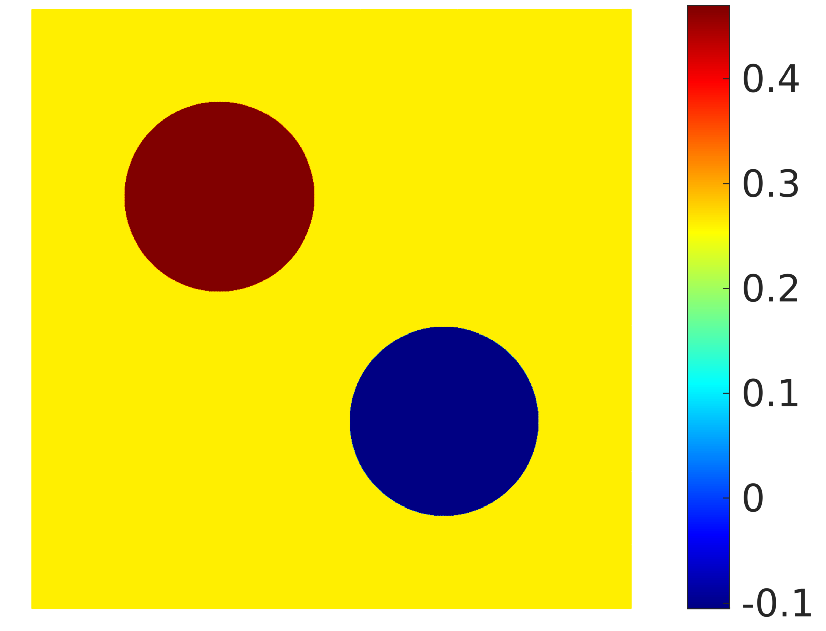
\includegraphics[width = 0.4\textwidth]{figures/sigma_exact}
	\caption{Plot of the exact unknown $\sigma^*$}.
	\label{fig:exact_unknown}
\end{figure}

One can verify that the tensor $A^{\varepsilon}_{\sigma}$ satisfies Assumption \ref{ass_A}. In particular, for $\xi \in \R^2$ we have
\begin{equation*}
A^{\varepsilon}_{\sigma} \xi \cdot \xi = a_{1,1} \left ( \sigma(x), \frac{x}{\varepsilon} \right ) \xi_1^2 + a_{2,2} \left ( \sigma(x), \frac{x}{\varepsilon} \right ) \xi_2^2 \ge e^{\sigma(x)} ( \xi_1^2 + \xi_2^2 ) = e^{\sigma_-} \norm{\xi}_2^2.
\end{equation*}
Moreover, since the $\mathrm{EnKF}$ algorithm estimates the coefficients $u$ of the truncated Karhunen-Lo\`eve expansion, we can show that for all $u_1, u_2 \in \R^M$
\begin{equation*}
\norm{A^{\varepsilon}(u_1) - A^{\varepsilon}(u_2)}_{L^{\infty}(\Omega, \R^{d \times d})} \le M \norm{u_1 - u_2}_2,
\end{equation*}
where $A^{\varepsilon}(u) = A^{\varepsilon}_{\sigma_u}$ and $\norm{\cdot}_2$ stands for the $2$-norm of a vector in $\R^M$. We have
\begin{align*}
& \norm{A^{\varepsilon}(u_1) - A^{\varepsilon}(u_2)}_{L^{\infty}(\Omega, \R^{d \times d})} =  \sup_{x \in \Omega} \sup_{\xi \in \R^2, \norm{\xi}_2=1} \norm{(A^{\varepsilon}(u_1) - A^{\varepsilon}(u_2)) \xi}_2 \\
& \qquad \le \sup_{x \in \Omega} \sqrt{\left ( a_{1,1} \left ( \sigma_{u_1}(x), \frac{x}{\varepsilon} \right ) - a_{1,1} \left ( \sigma_{u_2}(x), \frac{x}{\varepsilon} \right ) \right )^2 + \left ( a_{2,2} \left ( \sigma_{u_1}(x), \frac{x}{\varepsilon} \right ) - a_{2,2} \left ( \sigma_{u_2}(x), \frac{x}{\varepsilon} \right ) \right )^2},
\end{align*}
which implies
\begin{align*}
\norm{A^{\varepsilon}(u_1) - A^{\varepsilon}(u_2)}_{L^{\infty}(\Omega, \R^{d \times d})} & \; \le \sup_{x \in \Omega} \sqrt{13 \left ( e^{\sigma_{u_1}(x)} - e^{\sigma_{u_2}(x)} \right )^2} \\
& \; \le \sup_{x \in \Omega} \sqrt{13} e^{\sigma^+} \abs{\sigma_{u_1}(x) - \sigma_{u_2}(x)}.
\end{align*}
Using the truncated Karhunen-Lo\`eve expansion we obtain
\begin{align*}
\norm{A^{\varepsilon}(u_2)}_{L^{\infty}(\Omega, \R^{d \times d})} \le & \; \sup_{x \in \Omega} \sqrt{13} e^{\sigma^+} \left | \sum_{m=1}^M \sqrt{\lambda_m} \varphi_m(x) (u_{1,m} - u_{2,m}) \right | \\
\le & \; \sup_{x \in \Omega} \sqrt{13} e^{\sigma^+} \left ( \sum_{m=1}^M \lambda_m \varphi_m(x)^2 \right )^{1/2} \left ( \sum_{m=1}^M (u_{1,m} - u_{2,m})^2 \right )^{1/2} \\
= & \; \sup_{x \in \Omega} \sqrt{13} e^{\sigma^+} \left ( \sum_{m=1}^M \lambda_m \varphi_m(x)^2 \right )^{1/2} \norm{u_1 - u_2}_2,
\end{align*}
and defining $M = \sup_{x \in \Omega} \sqrt{13} e^{\sigma^+} \left ( \sum_{m=1}^M \lambda_m \varphi_m(x)^2 \right )^{1/2}$ we get the result.

\subsection{Results}

In Figure \ref{fig:best_solution} we plot the estimation $\sigma_{\mathrm{EnKF}}$ after $10, 50, 250$ and $500$ iterations of the ensemble Kalman algorithm. We clearly see that the approximation gets better as the number of iterations increases and that convergence has been reached, indeed we do not note a significant difference between the last two plots. We point out that we obtain a quite good approximation of the real unknown $\sigma^*$ , indeed we are trying to recover a non-continuous function in the whole domain given only some observations at the boundary.

\begin{figure}[t]
\centering
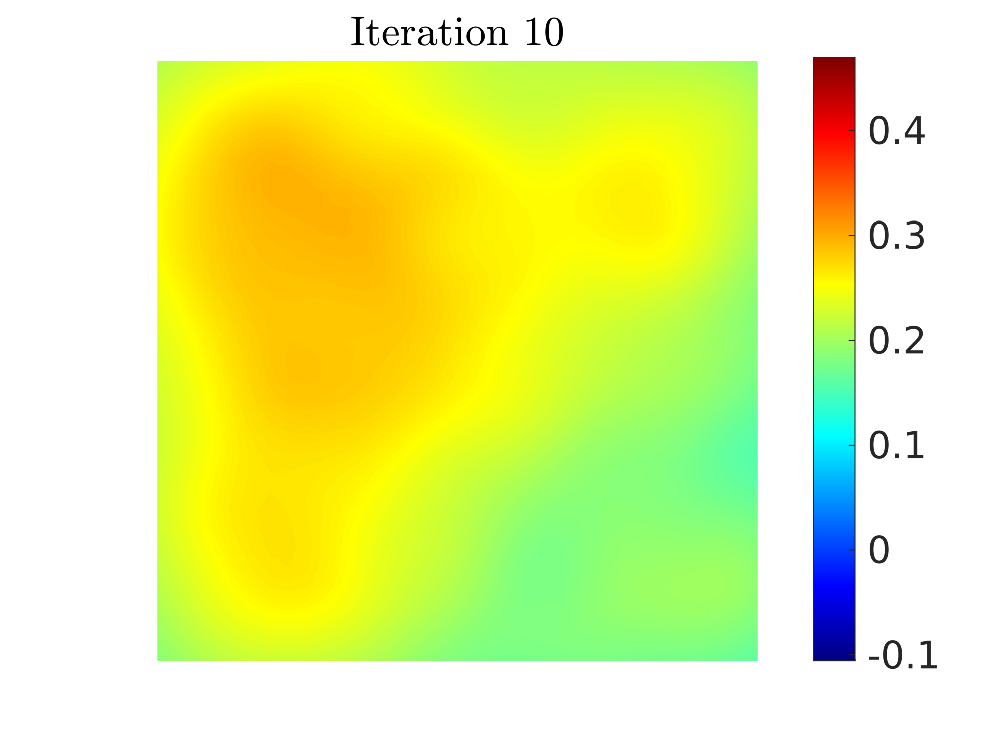
\includegraphics[width = 0.39\textwidth]{figures/ensemble_10}
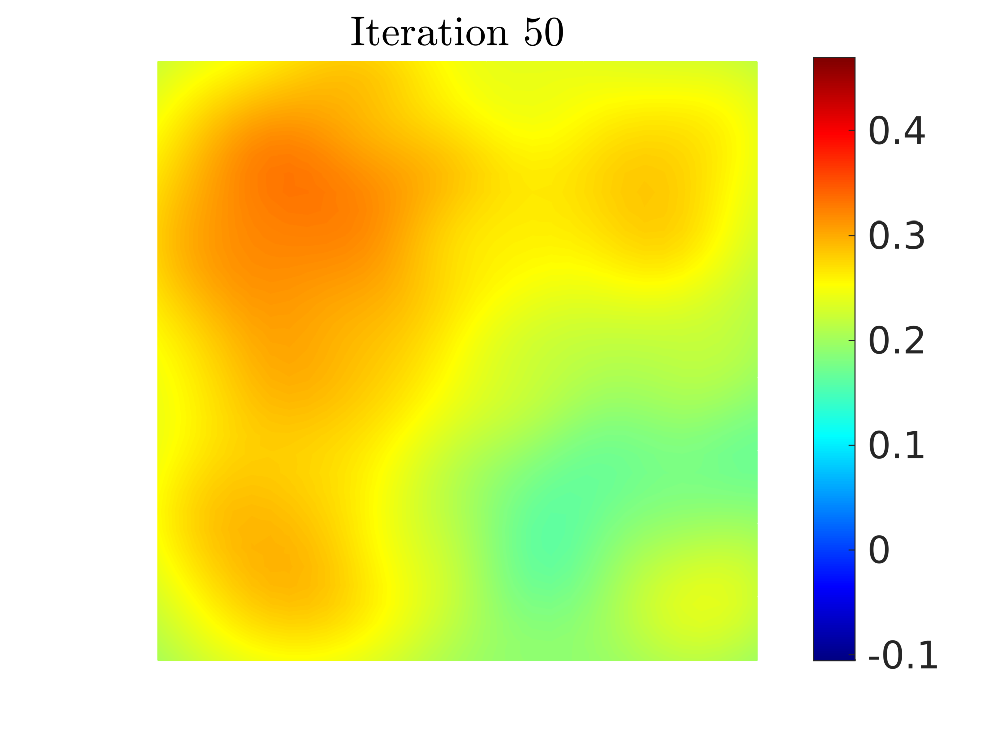
\includegraphics[width = 0.39\textwidth]{figures/ensemble_50}
\\
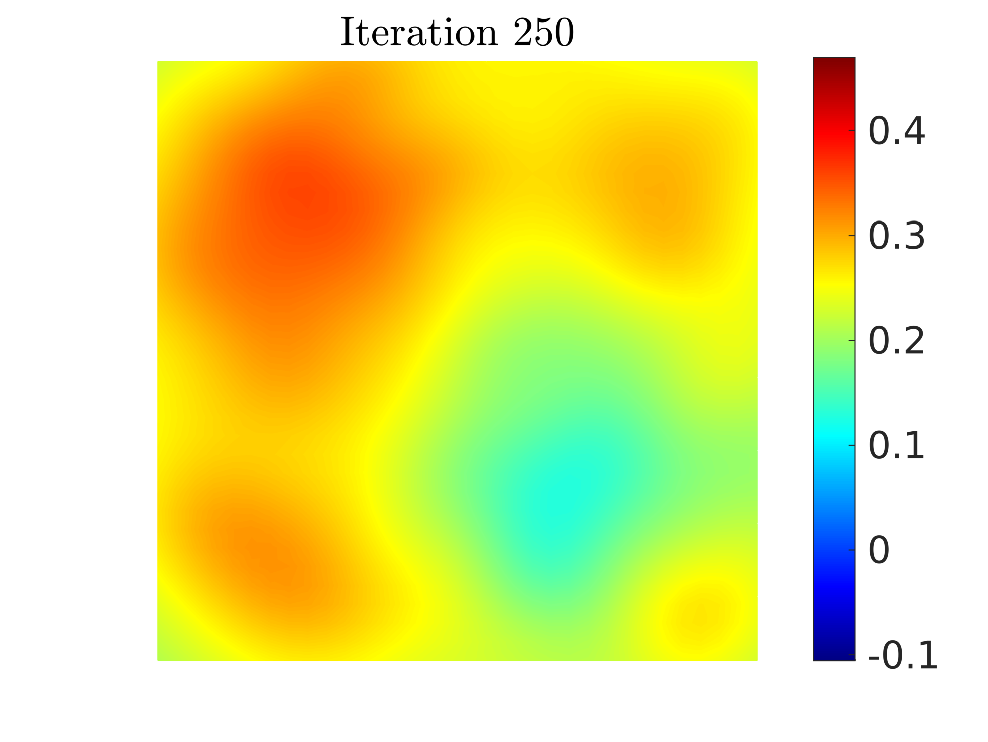
\includegraphics[width = 0.39\textwidth]{figures/ensemble_250}
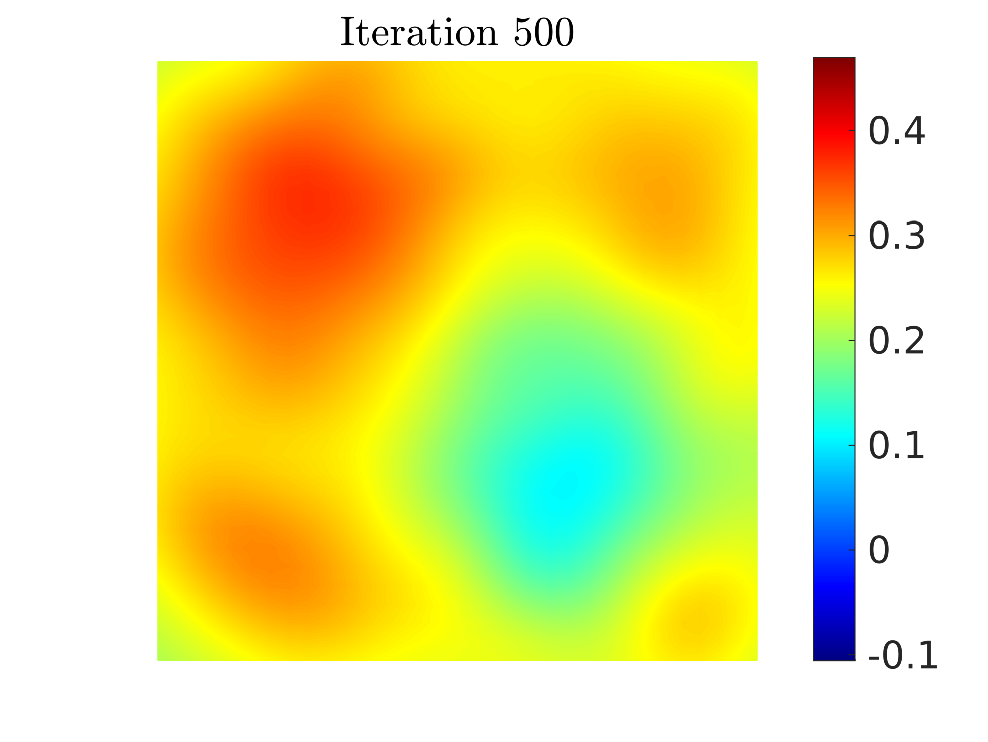
\includegraphics[width = 0.39\textwidth]{figures/ensemble_500}
\caption{Plot of the unknown $\sigma_{\mathrm{EnKF}}$ estimated by the iterative ensemble Kalman method after $10, 50, 250$ and $500$ iterations.}
\label{fig:best_solution}
\end{figure}

We perform a sensitivity analysis with respect to the dimension of the ensemble and the multiscale parameter $\varepsilon$. In Figure \ref{fig:comparison_J} we vary the number of particles $J$ and we compare the results obtained at the end of the algorithm after $500$ iterations. As expected, the approximation becomes better when the ensemble contains more particles. In particular, note that if the number of particles is too small, e.g. $J = 10$, then the approximation is completely different from the true unknown.

\begin{figure}[t]
\centering
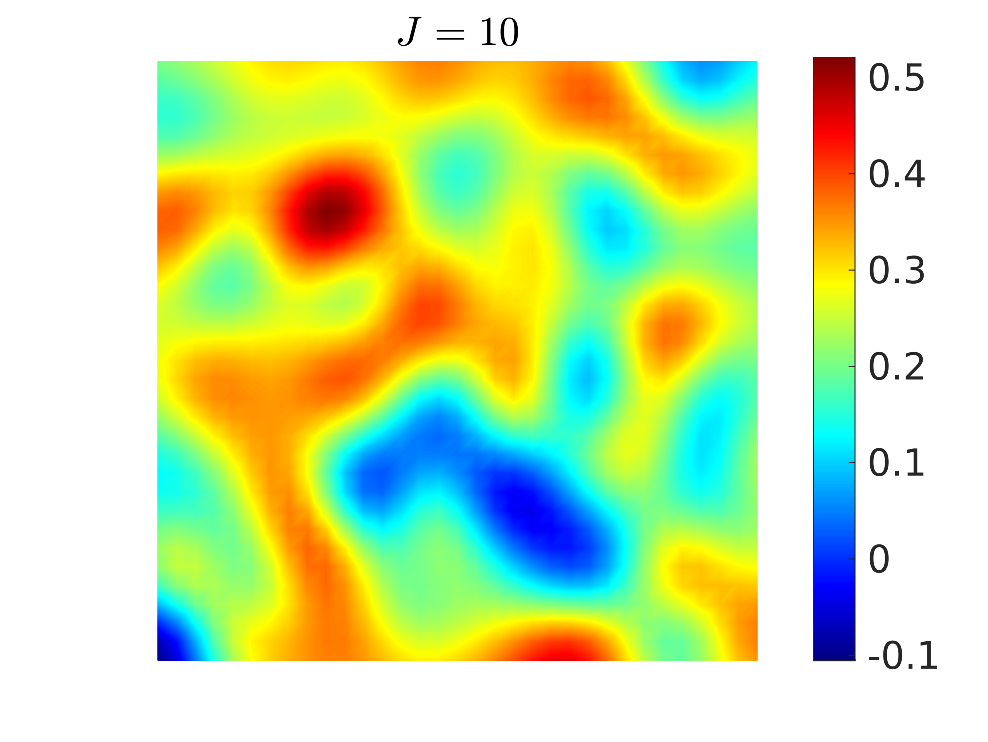
\includegraphics[width = 0.39\textwidth]{figures/ensemble_500_J10}
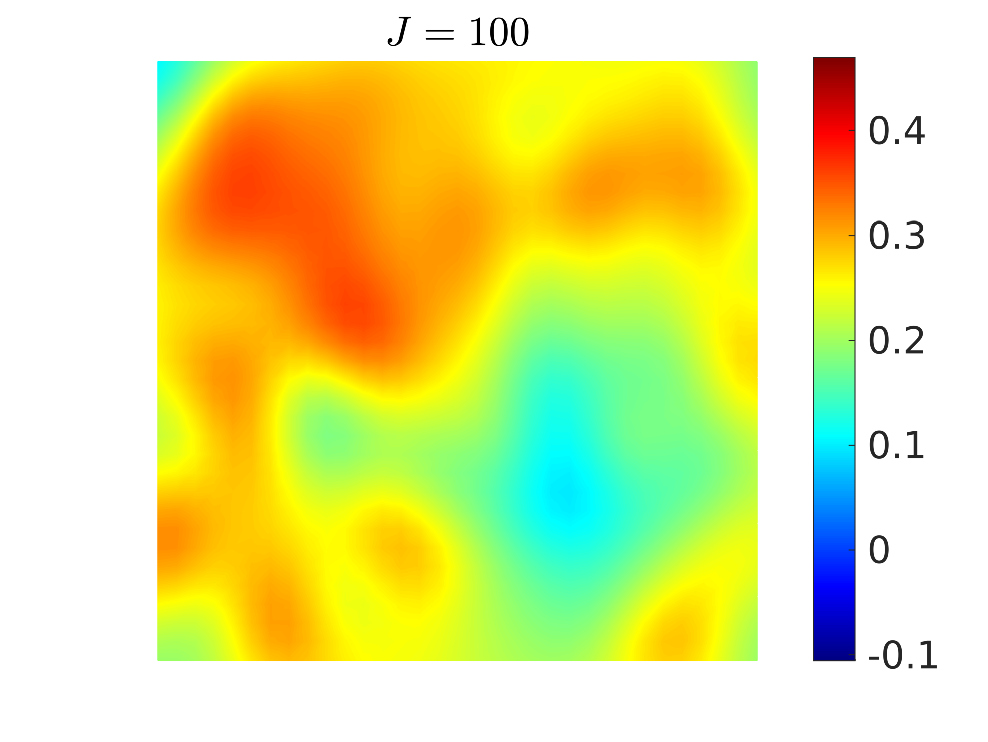
\includegraphics[width = 0.39\textwidth]{figures/ensemble_500_J100}
\\
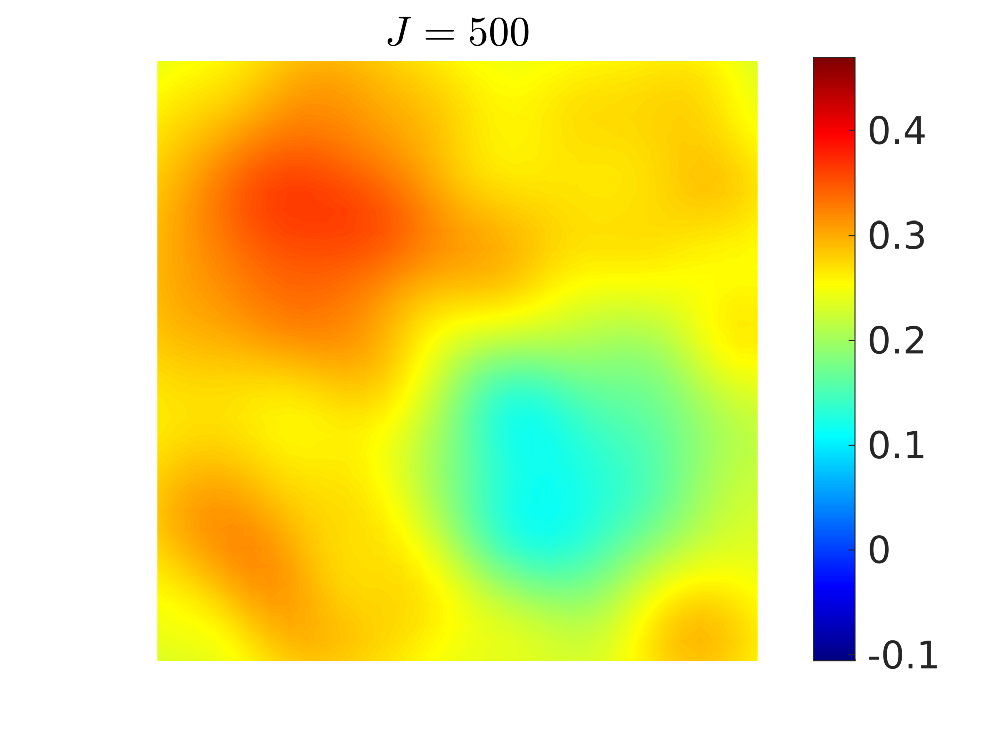
\includegraphics[width = 0.39\textwidth]{figures/ensemble_500_J500}
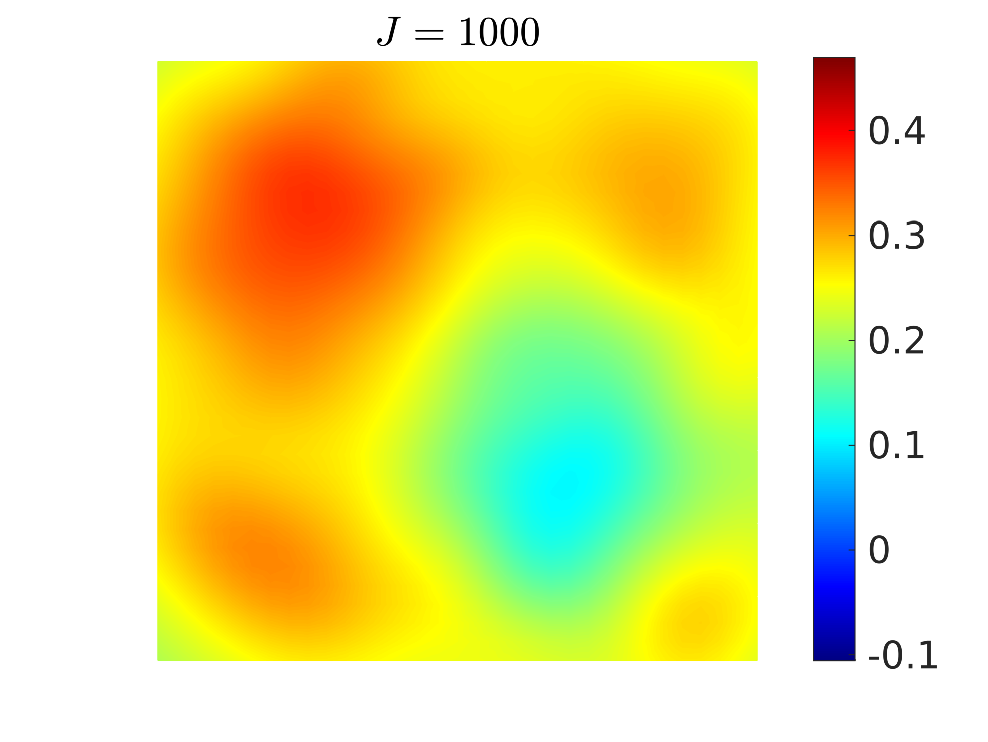
\includegraphics[width = 0.39\textwidth]{figures/ensemble_500_J1000}
\caption{Plot of the unknown $\sigma_{\mathrm{EnKF}}$ estimated by the iterative ensemble Kalman method after $500$ iterations for different numbers of particles per ensemble $J = 10, 100, 500, 1000$.}
\label{fig:comparison_J}
\end{figure}

In Figure \ref{fig:comparison_e} we compare the results obtained for different values of the multiscale parameter $\varepsilon$, in particular we take $\varepsilon = 1/4, 1/8, 1/32, 1/64$. We notice that the approximation becomes worse when $\varepsilon$ is bigger, indeed the homogenized problem becomes too different with respect to the multiscale one and, if $\varepsilon$ is too big, the solution does not approximate the true unknown.

\begin{figure}[t]
\centering
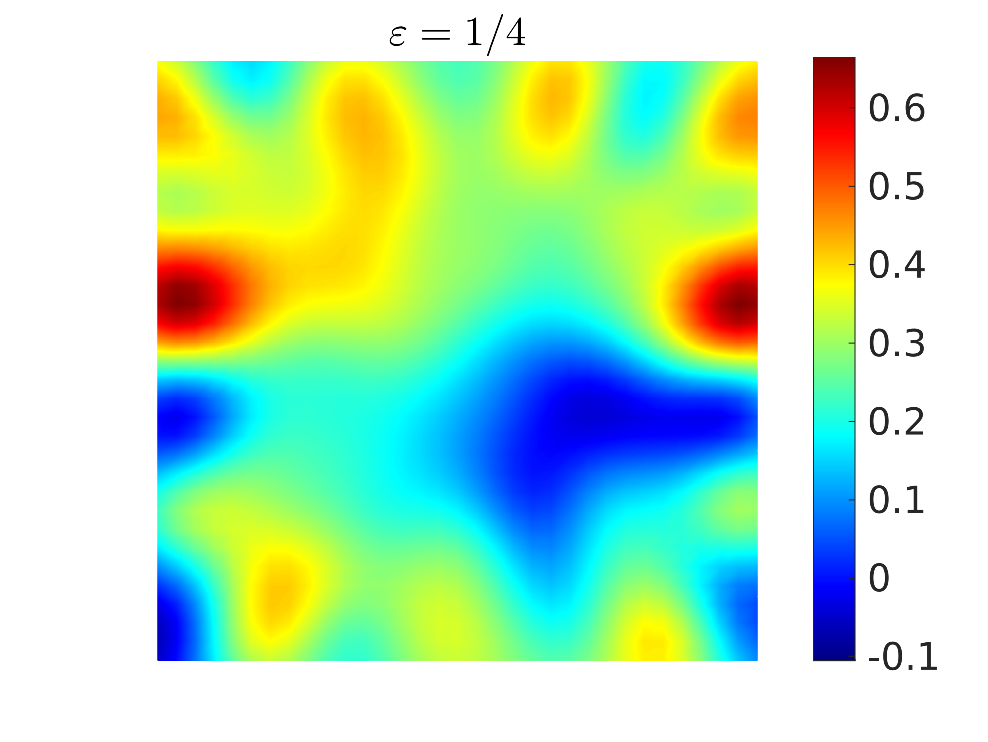
\includegraphics[width = 0.39\textwidth]{figures/ensemble_500_e4}
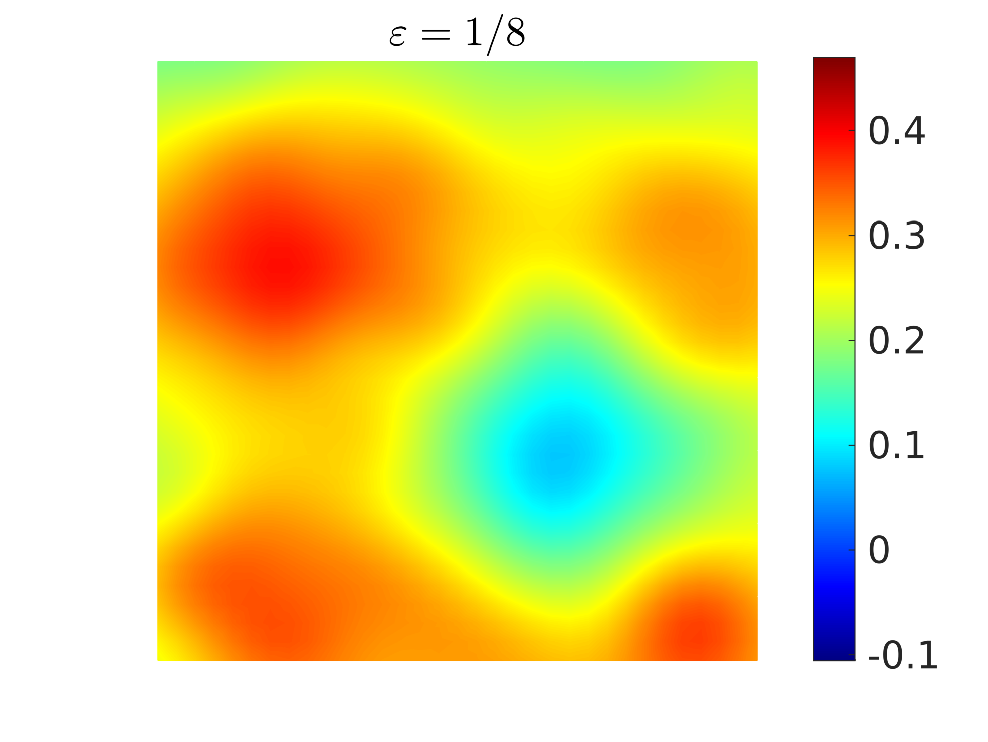
\includegraphics[width = 0.39\textwidth]{figures/ensemble_500_e8}
\\
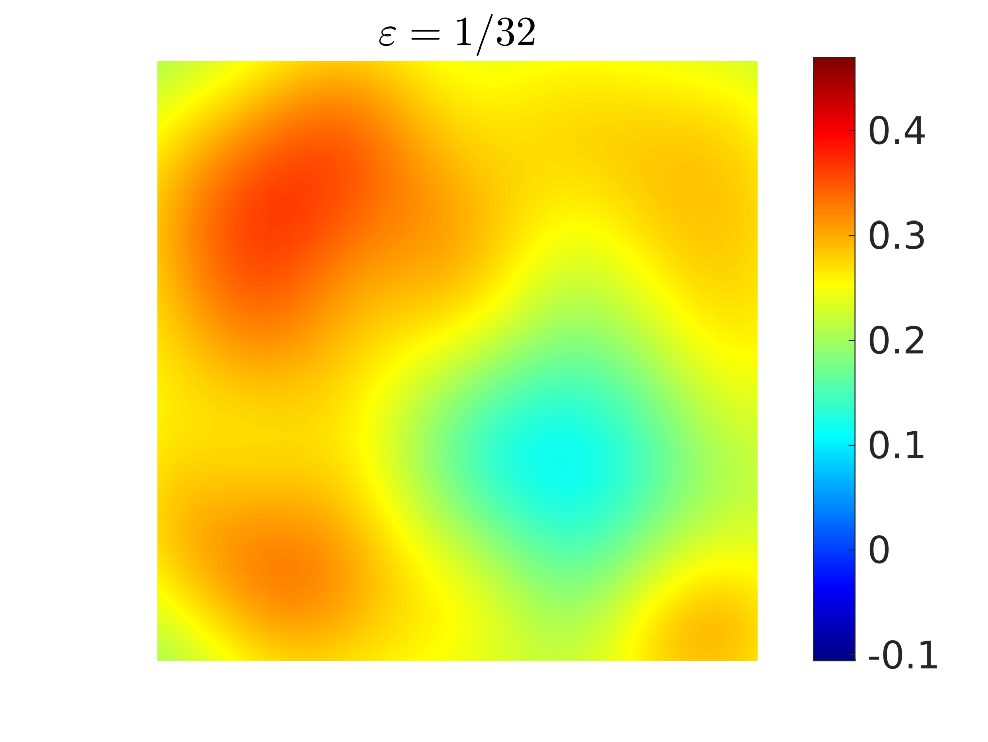
\includegraphics[width = 0.39\textwidth]{figures/ensemble_500_e32}
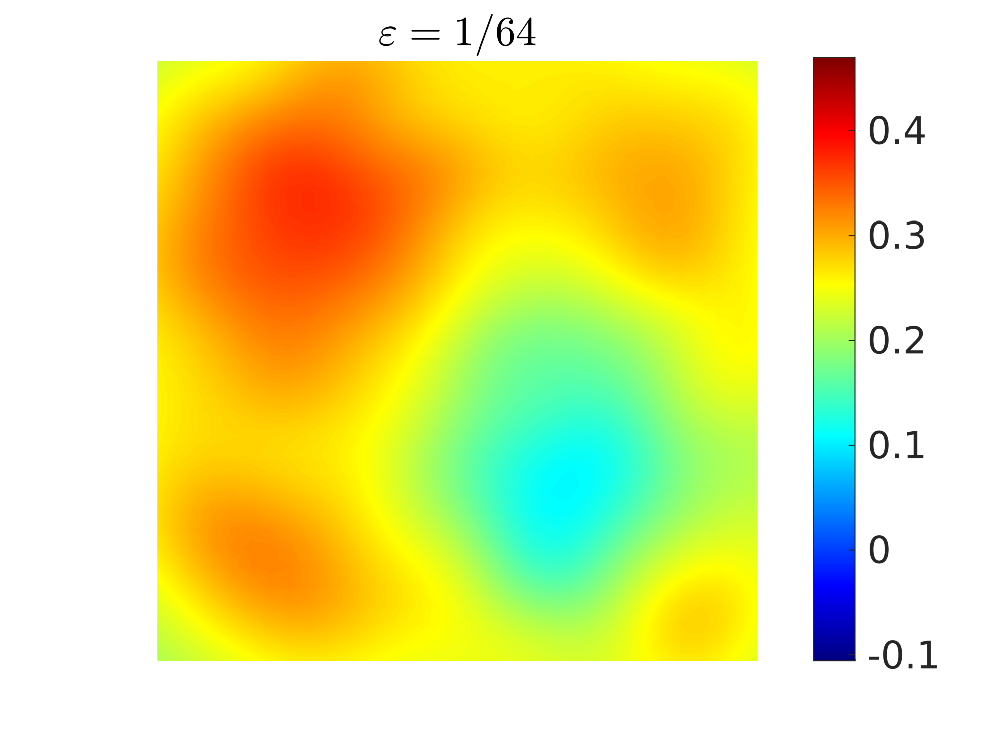
\includegraphics[width = 0.39\textwidth]{figures/ensemble_500_e64}
\caption{Plot of the unknown $\sigma_{\mathrm{EnKF}}$ estimated by the iterative ensemble Kalman method after $500$ iterations for different values of the multiscale parameter $\varepsilon = 1/4, 1/8, 1/32, 1/64$.}
\label{fig:comparison_e}
\end{figure}

Moreover, in order to obtain good results even in case $\varepsilon$ is not close to the asymptotic limit $\varepsilon \to 0$, in Figure \ref{fig:comparison_e_model_error} we apply offline modelling error estimation with $N_{\mathcal{E}} = 20$ and we plot the solution of the inverse problem \eqref{model_error_y4} for different values of the multiscale parameter $\varepsilon$. Comparing these plots with the ones in Figure \ref{fig:comparison_e}, in particular for $\varepsilon = 1/4$, we observe that the modelling error estimation significantly improves the results.

\begin{figure}[t]
\centering
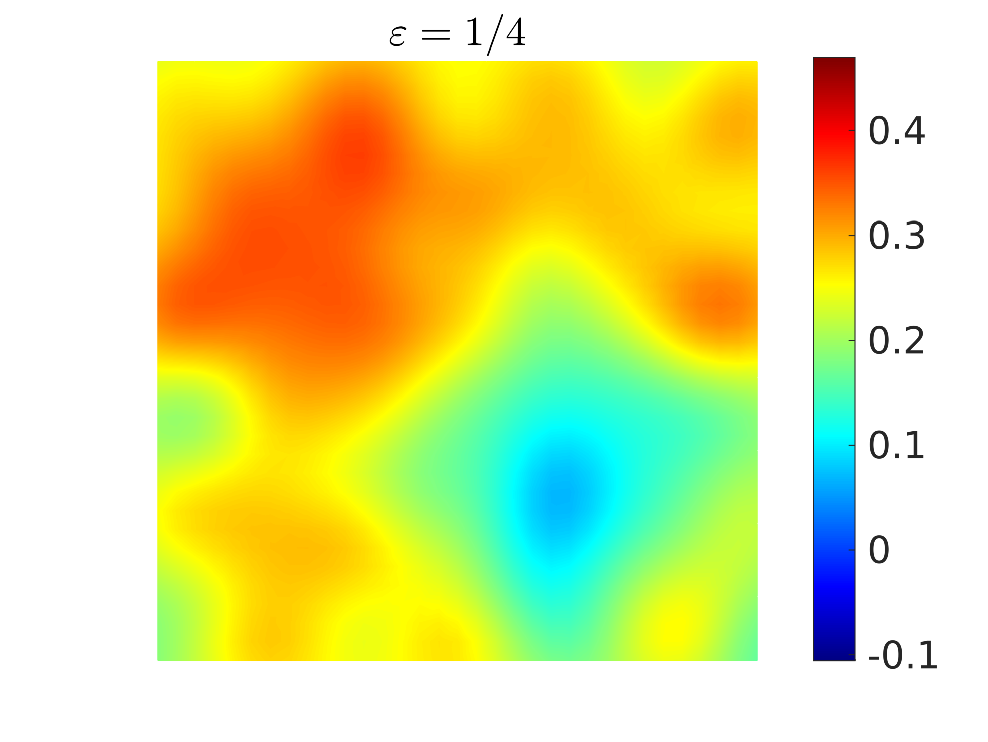
\includegraphics[width = 0.39\textwidth]{figures/ensemble_500_e4_model_error}
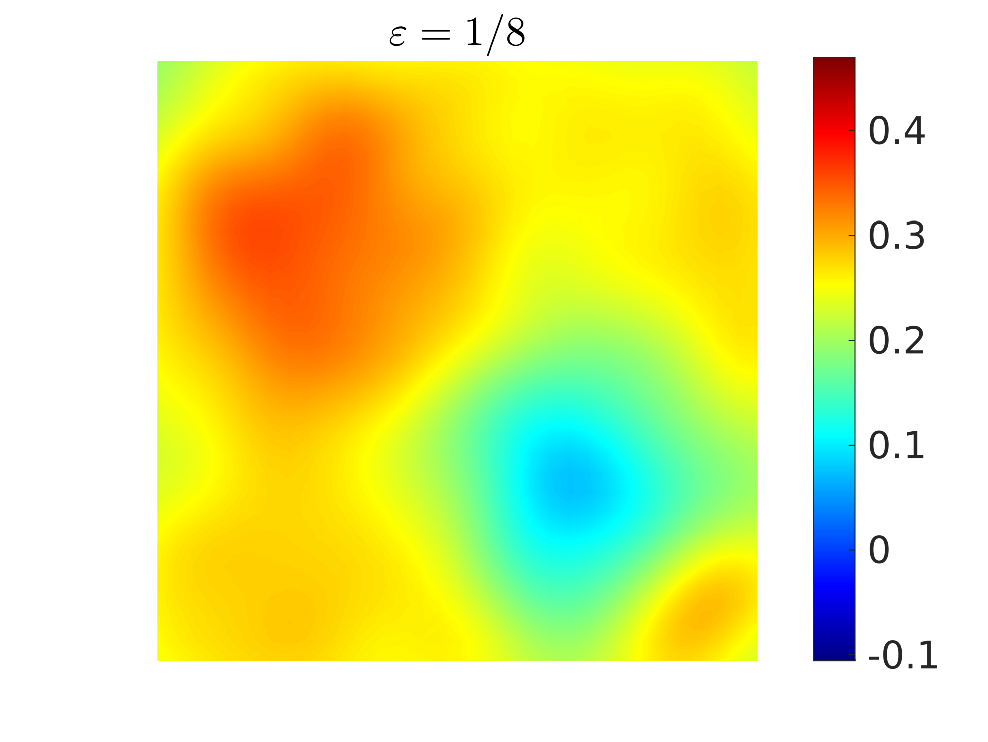
\includegraphics[width = 0.39\textwidth]{figures/ensemble_500_e8_model_error}
\\
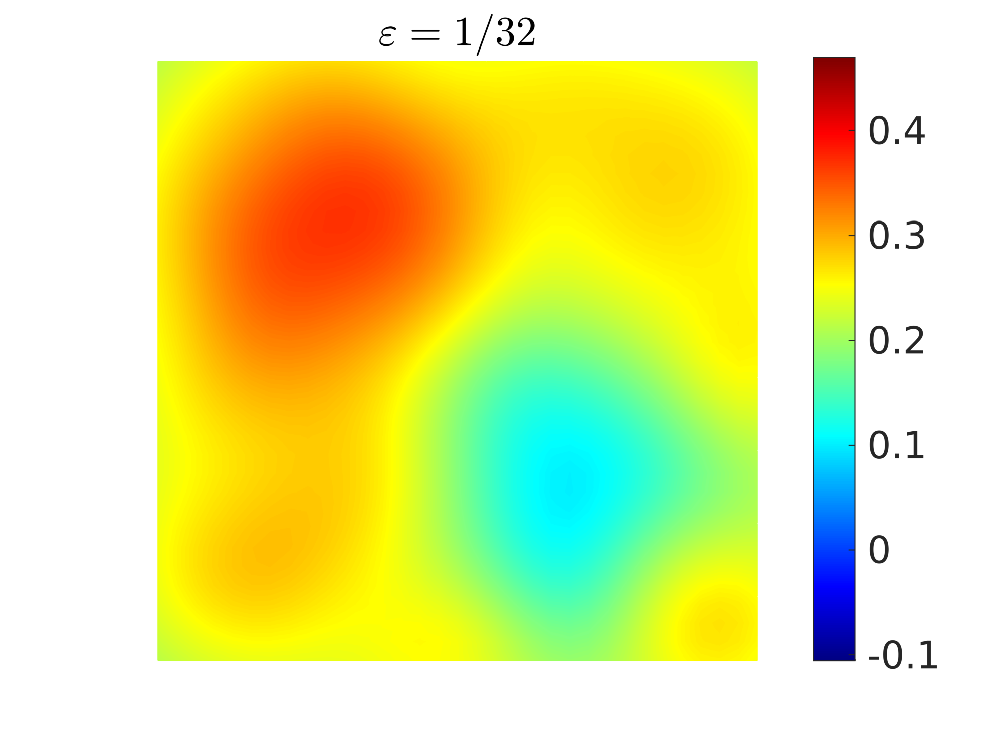
\includegraphics[width = 0.39\textwidth]{figures/ensemble_500_e32_model_error}
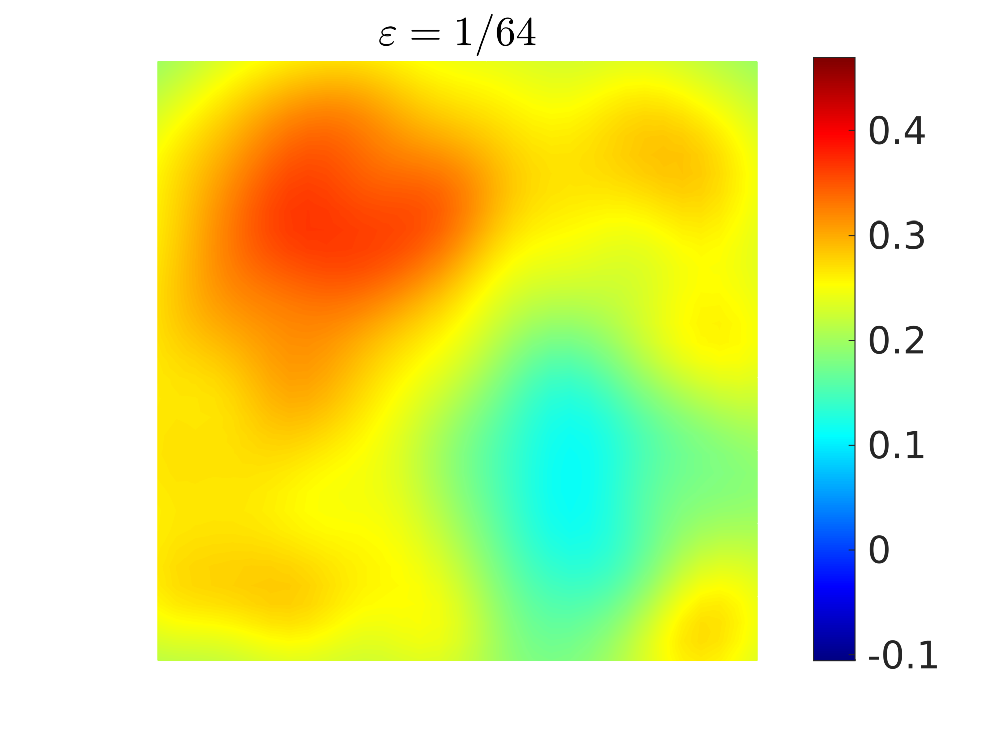
\includegraphics[width = 0.39\textwidth]{figures/ensemble_500_e64_model_error}
\caption{Plot of the unknown $\sigma_{\mathrm{EnKF}}$ estimated by the iterative ensemble Kalman method with model error estimation after $500$ iterations for different values of the multiscale parameter $\varepsilon = 1/4, 1/8, 1/32, 1/64$.}
\label{fig:comparison_e_model_error}
\end{figure}

Finally, in Figure \ref{fig:comparison_e_model_error_levels} we show the results obtained by applying the ensemble Kalman method with dynamic updating of the modelling error distribution with $\mathcal{L} = 5$ levels, $N_{\mathcal{E}}^{\ell} = 4$ samples and $N^{\ell} = 100$ iterations at each level $\ell = 1, \dots, \mathcal{L}$. The number of resolutions of the full multiscale problem is $20$ and the total number of iterations is $500$, which are equal to the previous approach, where the distribution of the modelling error was approximated offline. Comparing these plots with the ones in Figure \ref{fig:comparison_e_model_error}, we note that updating the distribution of the modelling error dynamically still improves the results.

\begin{figure}[t]
\centering
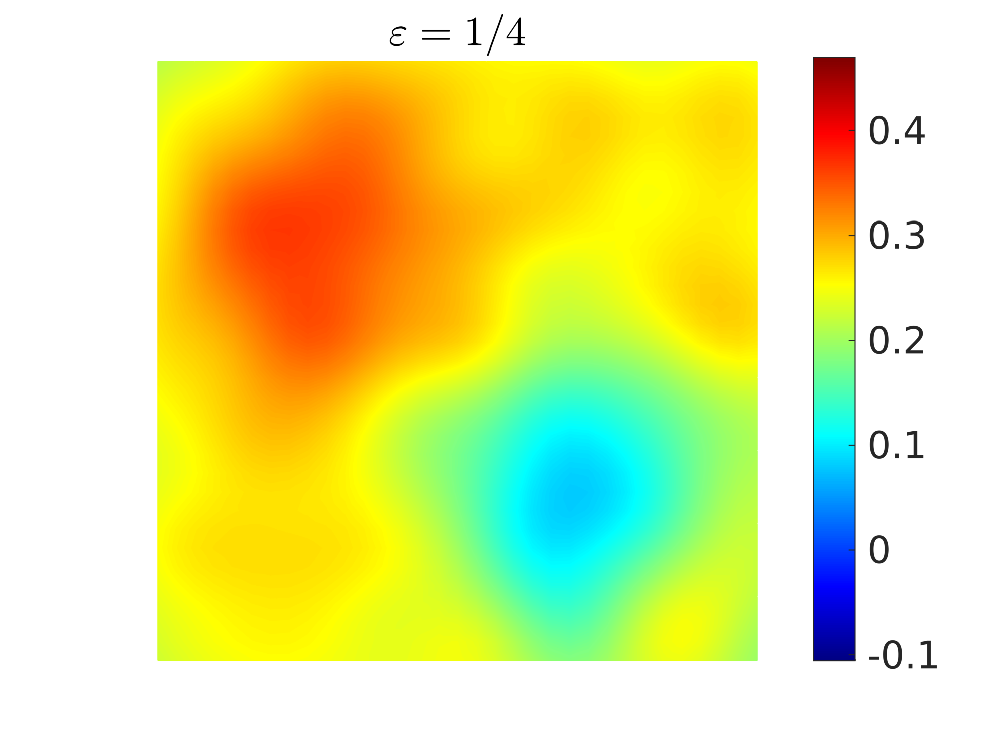
\includegraphics[width = 0.39\textwidth]{figures/ensemble_500_e4_model_error_Levels}
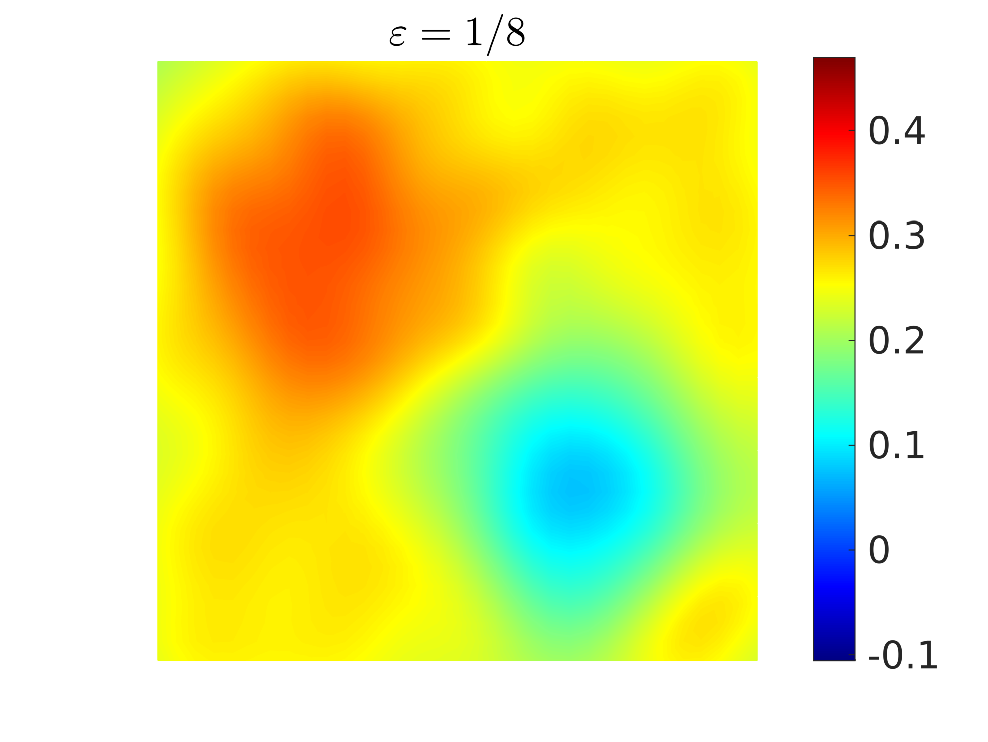
\includegraphics[width = 0.39\textwidth]{figures/ensemble_500_e8_model_error_Levels}
\\
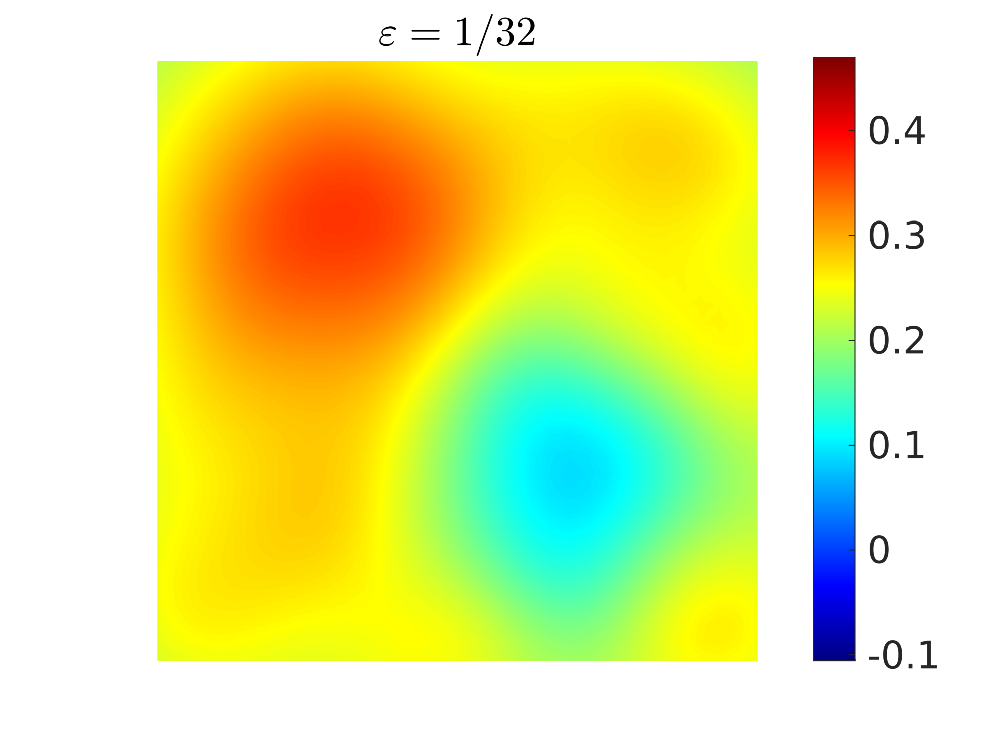
\includegraphics[width = 0.39\textwidth]{figures/ensemble_500_e32_model_error_Levels}
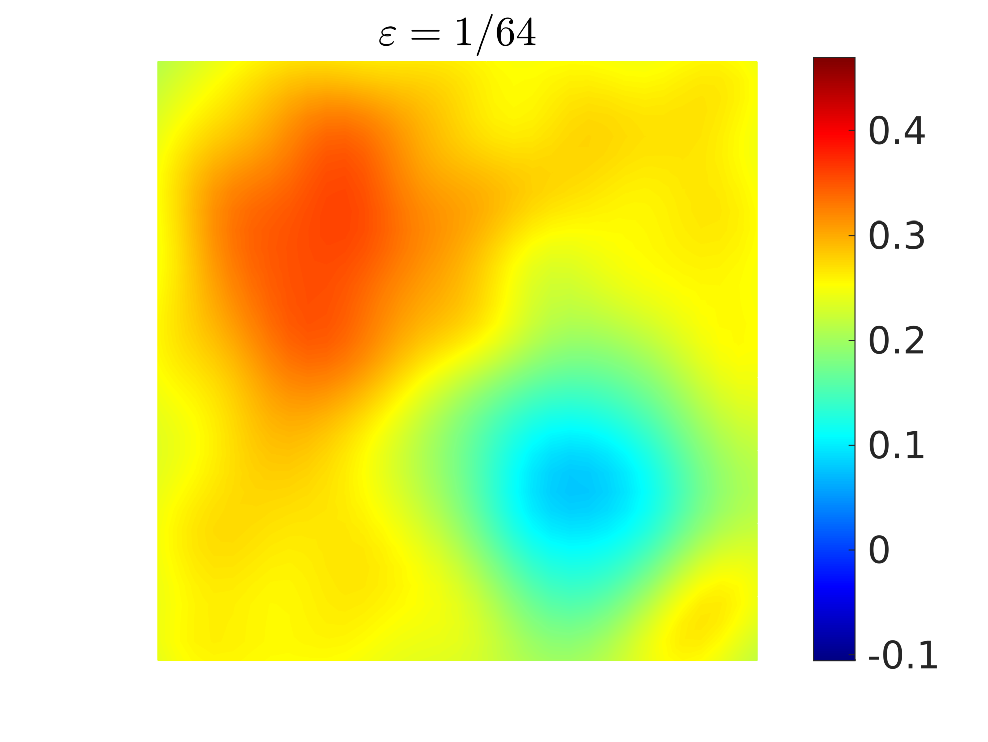
\includegraphics[width = 0.39\textwidth]{figures/ensemble_500_e64_model_error_Levels}
\caption{Plot of the unknown $\sigma_{\mathrm{EnKF}}$ estimated by the iterative ensemble Kalman method with dynamic updating of the model error estimation after $500$ iterations for different values of the multiscale parameter $\varepsilon = 1/4, 1/8, 1/32, 1/64$.}
\label{fig:comparison_e_model_error_levels}
\end{figure}

\section*{Conclusion}


\clearpage

\section*{Appendix}

\subsection*{Proof of Lemma \ref{lemma_difference_inverse}}

Note that
\[ A^{-1} - B^{-1} = A^{-1} (I - A B^{-1}) = A^{-1} (B - A) B^{-1}, \]
therefore we have
\[ \norm{A^{-1} - B^{-1}}_2 \le \norm{A^{-1}}_2 \norm{B - A}_2 \norm{B^{-1}}_2, \]
which is the desired result.

\qed

\subsection*{Proof of Lemma \ref{lemma_inverse_sum}}

Let $n$ be the dimension of the matrices, since $A$ is symmetric positive semidefinite and $B$ is symmetric positive definite, then $A + B$ is symmetric positive definite, and the eigenvalues of $A + B$ and $B$ are real and positive, thus they can be written
\[ 0 < \lambda_1(\cdot) \le \lambda_2(\cdot) \le \dots \le \lambda_n(\cdot), \]
counted with their multiplicity.
First, notice that, using the Rayleigh quotient and the fact that $x^T A x \ge 0$ for all $x$, we have
\[ \lambda_1(A + B) = \min_{x \neq 0} \frac{x^T(A + B)x}{x^T x} = \min_{x \neq 0} \frac{x^T A x + x^T B x}{x^T x} \ge \min_{x \neq 0} \frac{x^T B x}{x^T x} = \lambda_1(B), \]
which implies
\[ \norm{(A + B)^{-1}}_2 = \frac{1}{\lambda_1(A + B)} \le \frac{1}{\lambda_1(B)} = \norm{B^{-1}}_2, \]
which is the desired result.

\qed

\subsection*{Proof of Lemma \ref{G_lipschitz}}

Let $u_1, u_2 \in \mathbb{R}^M$, \corr{and $p_1 = \mathcal S(u_1)$, $p_2 = \mathcal S(u_2)$ Then, writing the weak formulations of \eqref{problem_lemma} we get
	\begin{equation*}
	\int_\Omega \big(A(u_1)\nabla p_1 - A(u_2) \nabla p_2\big) \cdot \nabla v = 0,	
	\end{equation*}
	for all $v \in H^1_0(\Omega)$. Adding and subtracting $A(u_1) \nabla p_2$ to the first factor inside the integral and rearranging terms yields}
\begin{equation*}
\int_{\Omega} A(u_1) (\nabla p_1 - \nabla p_2) \cdot \nabla v = - \int_{\Omega} (A(u_1) - A(u_2)) \nabla p_2 \cdot \nabla v.
\end{equation*}
\corr{Choosing $v = p_1 - p_2$,} using the hypotheses on $A$ and the H\"older inequality, we obtain
\begin{align*}
\alpha \norm{\nabla p_1 - \nabla p_2}_{L^2(\Omega; \R^d)}^2 \le & \;  \int_{\Omega} \left | (A(u_1) - A(u_2)) \nabla p_2 \cdot (\nabla p_1 - \nabla p_2) \right | \\
\le & \; \norm{A(u_1) - A(u_2)}_{L^{\infty}(\Omega; \R^{d \times d})} \norm{\nabla p_2}_{L^2(\Omega; \R^d)} \norm{\nabla p_1 - \nabla p_2}_{L^2(\Omega; \R^d)} \\
\le & \; M \norm{u_1 - u_2}_2 \norm{\nabla p_2}_{L^2(\Omega; \R^d)} \norm{\nabla p_1 - \nabla p_2}_{L^2(\Omega; \R^d)},
\end{align*}
which implies 
\begin{equation} \label{intermediate}
\norm{\nabla p_1 - \nabla p_2}_{L^2(\Omega; \R^d)} \le \frac{M}{\alpha} \norm{\nabla p_2}_{L^2(\Omega; \R^d)} \norm{u_1 - u_2}_2.
\end{equation}
\corr{It remains} to bound $\norm{\nabla p_2}_{L^2(\Omega; \R^N)}$, \corr{which can be achieved with a standard coercivity argument. In particular, we have
	\begin{equation} 
	\norm{\nabla p_2}_{L^2(\Omega; \R^N)} \le \frac{C_p}{\alpha} \norm{f}_{L^2(\Omega)}, 
	\end{equation}
	where $C_p$ is the Poincaré constant associated to the domain $\Omega$. Replacing in \eqref{intermediate}}, we obtain
\begin{equation*}
\norm{\nabla p_1 - \nabla p_2}_{L^2(\Omega; \R^N)} \le \frac{M C_p}{\alpha^2} \norm{f}_{L^2(\Omega)} \norm{u_1 - u_2}_2 = L_{\mathcal{S}} \norm{u_1 - u_2}_2,
\end{equation*}
which shows that $\mathcal{S}$ is Lipschitz with constant
\[ L_{\mathcal{S}} = \frac{M C_p}{\alpha^2} \norm{f}_{L^2(\Omega)}. \]
Finally, $\mathcal{G}$ is the composition of two Lipschitz operators, so it is Lipschitz \corr{of constant $L_{\mathcal G} = L_{\mathcal O} L_{\mathcal S}$}, which concludes the proof.
\qed

%\subsection*{Proof of Lemma \ref{wH1_sL2}}
%
%The sequence $\{ p^{\varepsilon} \}$ is weakly convergent in $H^1_0(\Omega)$, hence it is bounded in $H^1_0(\Omega)$. By Rellich theorem, $H^1_0(\Omega)$ is compactly embedded in $L^2(\Omega)$, so there exists a subsequence $\{ p^{\varepsilon'} \}$ such that
%\[ p^{\varepsilon'} \to \bar{p} \qquad \text{in } L^2(\Omega) \]
%for some $\bar{p}$ in $L^2(\Omega)$. Strong convergence implies weak convergence, therefore we obtain 
%\begin{equation}
%\label{convergence_pbar}
%p^{\varepsilon'} \toweak \bar{p} \qquad \text{in } L^2(\Omega).
%\end{equation}
%Moreover, since $p^{\varepsilon} \toweak p^0$ in $H^1_0(\Omega)$, we also have that this is true for the subsequence $p^{\varepsilon'}$
%\[ p^{\varepsilon'} \toweak p^0 \qquad \text{in } H^1_0(\Omega), \]
%which implies
%\begin{equation}
%\label{convergence_p0}
%p^{\varepsilon'} \toweak p^0 \qquad \text{in } L^2(\Omega).
%\end{equation}
%Thanks to (\ref{convergence_pbar}) and (\ref{convergence_p0}) and by uniqueness of the weak limit we deduce that $\bar{p} = p^0$, thus
%\[ p^{\varepsilon'} \to p^0 \qquad \text{in } L^2(\Omega). \]
%Finally, repeating this argument for subsequences, we deduce that every subsequence admits a sub-subsequence strongly converging to the same limit in $L^2(\Omega)$, hence the whole sequence strongly
%converges to $p^0$, that is
%\[ p^{\varepsilon} \to p^0 \qquad \text{in } L^2(\Omega), \]
%which is the desired result.
%
%\qed

\subsection*{Proof of Lemma \ref{f_goes_to_0}}

Let us consider an ensemble $u \in \mathcal U_{J,M}$ with particles $u^{(j)} \in \R^M$, for $j = 1, \ldots, J$. For each particle we have
\begin{align}
\norm{\mathcal{G}^{\varepsilon}(u^{(j)}) - \mathcal{G}^0(u^{(j)})}_2 = & \; \norm{\mathcal{O}(\mathcal{S}^{\varepsilon}(u^{(j)})) - \mathcal{O}(\mathcal{S}^0(u^{(j)}))}_2 \\
= & \; \norm{\mathcal{O}(p^{\varepsilon}(u^{(j)})) - \mathcal{O}(p^0(u^{(j)}))}_2 \\
\le & \; m \norm{p^{\varepsilon}(u^{(j)}) - p^0(u^{(j)})}_{L^2(\Omega)},
\end{align}
where we write explicitly the dependence of $p^{\varepsilon}$ and $p^0$ on the particle it is generated by.
By homogenization theory, we know that $p^{\varepsilon}(u^{(j)}) \toweak p^0(u^{(j)})$ in $H^1_0(\Omega)$, and therefore we have $p^{\varepsilon}(u^{(j)}) \to p^0(u^{(j)})$ in $L^2(\Omega)$, which implies
\[ e(\varepsilon, u) = \frac{1}{J} \sum_{j=1}^J \norm{\mathcal{G}^{\varepsilon}(u^{(j)}) - \mathcal{G}^0(u^{(j)})}_2 \to 0. \]
Moreover, if the solution of the homogenized problem $p^0$ is sufficiently smooth independently of $u$, namely $p^0 \in H^2(\Omega)$, letting $C > 0$ be a constant, we have for all $j = 1, \dots, J$ the following estimate, which can be found in \cite{Gri05}
\[ \norm{p^{\varepsilon}(u^{(j)}) - p^0(u^{(j)})}_{L^2(\Omega)} \le C \varepsilon, \]
hence we finally obtain
\[ e(\varepsilon, u) = \frac{1}{J} \sum_{j=1}^J \norm{\mathcal{G}^{\varepsilon}(u^{(j)}) - \mathcal{G}^0(u^{(j)})}_2 \le m C \varepsilon, \]
which proves the result for $K = m C$.

\qed

\subsection*{Proof of Lemma \ref{covariance_bound}}

Let $L$ be the Lipschitz constant of $\mathcal{G}$. For all $x \in B_R(u^*)$ we have
\begin{align*}
& \norm{\mathcal{G}(x)}_2 \le \norm{\mathcal{G}(x) - \mathcal{G}(u^*)}_2 + \norm{\mathcal{G}(u^*)}_2 \le L \norm{x - u^*}_2 + \norm{\mathcal{G}(u^*)}_2 \le LR + G, \\
& \norm{x}_2 \le \norm{x - u^*}_2 + \norm{u^*}_2 \le R + g,
\end{align*}
and we define the bounds $M = LR + G$ and $m = R + g$. The same bounds can be deduced for the mean values
\begin{align}
\label{bound_mean_u}
& \norm{\bar{u}}_2 \le \frac{1}{J} \sum_{j=1}^J \norm{u^{(j)}}_2 \le \frac{1}{J} J m = m, \\
\label{bound_mean_G}
& \norm{\bar{\mathcal{G}}}_2 \le \frac{1}{J} \sum_{j=1}^J \norm{\mathcal{G}(u^{(j)})}_2 \le \frac{1}{J} J M = M.
\end{align}
By definition of $2$-norm of a matrix we have
\begin{align*}
\norm{C^{up}(u)}_2 = & \; \sup_{x \in \mathbb{R}^L \colon \norm{x}_2 = 1} \left \lVert \frac{1}{J} \sum_{j=1}^J (u^{(j)} - \bar{u}) (\mathcal{G}(u^{(j)}) - \bar{\mathcal{G}})^T x \right \rVert_2 \\
\le & \; \sup_{x \in \mathbb{R}^L \colon \norm{x}_2 = 1} \frac{1}{J} \sum_{j=1}^J \left | (\mathcal{G}(u^{(j)}) - \bar{\mathcal{G}})^T x \right | \norm{u^{(j)} - \bar{u}}_2 \\
\le & \; \sup_{x \in \mathbb{R}^L \colon \norm{x}_2 = 1} \frac{1}{J} \sum_{j=1}^J \left \lVert \mathcal{G}(u^{(j)}) - \bar{\mathcal{G}} \right \rVert_2 \norm{x}_2 \norm{u^{(j)} - \bar{u}}_2,
\end{align*}
and using (\ref{bound_mean_u}) and (\ref{bound_mean_G}) and the fact that $\norm{x}_2 = 1$ we obtain
\begin{align*}
\norm{C^{up}(u)}_2 \le & \; \frac{1}{J} \sum_{j=1}^J \left ( \norm{\mathcal{G}(u^{(j)})}_2 + \norm{\bar{\mathcal{G}}}_2 \right ) \left ( \norm{u^{(j)}}_2 + \norm{\bar{u}}_2 \right ) \\
\le & \; \frac{1}{J} J (M + M) (m + m) = 4Mm,
\end{align*}
and we define $C_1 = 4Mm$.
The procedure is similar for the matrix $C^{pp}(u)$, where we have
\begin{align*}
\norm{C^{pp}(u)}_2 = & \; \sup_{x \in \mathbb{R}^L \colon \norm{x}_2 = 1} \left \lVert \frac{1}{J} \sum_{j=1}^J (\mathcal{G}(u^{(j)}) - \bar{\mathcal{G}}) (\mathcal{G}(u^{(j)}) - \bar{\mathcal{G}})^T x \right \rVert_2 \\
\le & \; \sup_{x \in \mathbb{R}^L \colon \norm{x}_2 = 1} \frac{1}{J} \sum_{j=1}^J \left | (\mathcal{G}(u^{(j)}) - \bar{\mathcal{G}})^T x \right | \left \lVert \mathcal{G}(u^{(j)}) - \bar{\mathcal{G}} \right \rVert_2 \\
\le & \; \sup_{x \in \mathbb{R}^L \colon \norm{x}_2 = 1} \frac{1}{J} \sum_{j=1}^J \left \lVert \mathcal{G}(u^{(j)}) - \bar{\mathcal{G}} \right \rVert^2_2 \norm{x}_2,
\end{align*}
and using bound (\ref{bound_mean_G}) and the fact that $\norm{x}_2 = 1$ we obtain
\begin{align*}
\norm{C^{up}(u)}_2 \le & \; \frac{1}{J} \sum_{j=1}^J \left ( \norm{\mathcal{G}(u^{(j)})}_2 + \norm{\bar{\mathcal{G}}}_2 \right )^2 \\
\le & \; \frac{1}{J} J (M + M)^2 = 4M^2,
\end{align*}
and we define $C_2 = 4M^2$. \\
Before proving the last two results of the lemma we need the following estimates for the ensemble of particles $u_1$ and $u_2$
\begin{align*}
\norm{\bar{u}_1 - \bar{u}_2}_2 = & \; \left \lVert \frac{1}{J} \sum_{j=1}^J (u_1^{(j)} - u_2^{(j)}) \right \rVert_2 \le \frac{1}{J} \sum_{j=1}^J \norm{u_1^{(j)} - u_2^{(j)}}_2 = \norm{u_1 - u_2}, \\
\norm{\bar{\mathcal{G}}_1 - \bar{\mathcal{G}}_2}_2 = & \; \left \lVert \frac{1}{J} \sum_{j=1}^J (\mathcal{G}(u_1^{(j)}) - \mathcal{G}(u_2^{(j)})) \right \rVert_2 \le \frac{1}{J} \sum_{j=1}^J \norm{\mathcal{G}(u_1^{(j)}) - \mathcal{G}(u_2^{(j)})}_2 \\
& \hspace{137pt} \le L \frac{1}{J} \sum_{j=1}^J \norm{u_1^{(j)} - u_2^{(j)}}_2 \\
& \hspace{137pt} = L \norm{u_1 - u_2}.
\end{align*}
By definition of $2$ norm of a matrix and using the triangle inequality we have
\begin{align*}
& \norm{C^{up}(u_1) - C^{up}(u_2)}_2 \\
& \qquad = \sup_{x \in \mathbb{R}^L \colon \norm{x}_2 = 1} \left \lVert \frac{1}{J} \sum_{j=1}^J \left [ (u_1^{(j)} - \bar{u}_1) (\mathcal{G}(u_1^{(j)}) - \bar{\mathcal{G}}_1)^T x - (u_2^{(j)} - \bar{u}_2) (\mathcal{G}(u_2^{(j)}) - \bar{\mathcal{G}}_2)^T x \right ] \right \rVert_2 \\
& \qquad \le \quad \sup_{x \in \mathbb{R}^L \colon \norm{x}_2 = 1} \frac{1}{J} \sum_{j=1}^J \left \lVert (u_1^{(j)} - \bar{u}_1) (\mathcal{G}(u_1^{(j)}) - \bar{\mathcal{G}}_1)^T x - (u_1^{(j)} - \bar{u}_1) (\mathcal{G}(u_2^{(j)}) - \bar{\mathcal{G}}_2)^T x \right \rVert_2 \\
& \qquad \quad + \sup_{x \in \mathbb{R}^L \colon \norm{x}_2 = 1} \frac{1}{J} \sum_{j=1}^J \left \lVert (u_1^{(j)} - \bar{u}_1) (\mathcal{G}(u_2^{(j)}) - \bar{\mathcal{G}}_2)^T x - (u_2^{(j)} - \bar{u}_2) (\mathcal{G}(u_2^{(j)}) - \bar{\mathcal{G}}_2)^T x \right \rVert_2,
\end{align*}
which implies
\begin{align*}
& \norm{C^{up}(u_1) - C^{up}(u_2)}_2 \\
& \qquad \le \quad \sup_{x \in \mathbb{R}^L \colon \norm{x}_2 = 1} \frac{1}{J} \sum_{j=1}^J \left \lVert (u_1^{(j)} - \bar{u}_1) [ (\mathcal{G}(u_1^{(j)}) - \mathcal{G}(u_2^{(j)})) + (\bar{\mathcal{G}}_2 - \bar{\mathcal{G}}_1)]^T x ] \right \rVert_2 \\
& \qquad \quad + \sup_{x \in \mathbb{R}^L \colon \norm{x}_2 = 1} \frac{1}{J} \sum_{j=1}^J \left \lVert [ (u_1^{(j)} - u_2^{(j)}) + (\bar{u}_2 - \bar{u}_1) ] (\mathcal{G}(u_2^{(j)}) - \bar{\mathcal{G}}_2)^T x \right \rVert_2 \\ 
& \qquad \le \quad \sup_{x \in \mathbb{R}^L \colon \norm{x}_2 = 1} \frac{1}{J} \sum_{j=1}^J \norm{u_1^{(j)} - \bar{u}_1}_2 [ \norm{\mathcal{G}(u_1^{(j)}) - \mathcal{G}(u_2^{(j)})}_2 + \norm{\bar{\mathcal{G}}_2 - \bar{\mathcal{G}}_1}_2 ] \norm{x}_2 \\
& \qquad \quad + \sup_{x \in \mathbb{R}^L \colon \norm{x}_2 = 1} \frac{1}{J} \sum_{j=1}^J [ \norm{u_1^{(j)} - u_2^{(j)}}_2 + \norm{\bar{u}_2 - \bar{u}_1}_2 ] \norm{\mathcal{G}(u_2^{(j)}) - \bar{\mathcal{G}}_2} \norm{x}_2.
\end{align*}
Using bounds (\ref{bound_mean_u}) and (\ref{bound_mean_G}) and the fact that $\mathcal{G}$ is Lipschitz with constant $L$, we obtain
\begin{align*}
& \norm{C^{up}(u_1) - C^{up}(u_2)}_2 \\
& \qquad \le \frac{1}{J} \sum_{j=1}^J \left \{ (\norm{u_1^{(j)}}_2 + \norm{\bar{u}_1}_2) (L \norm{u_1^{(j)} - u_2^{(j)}}_2 + L \norm{u_1 - u_2}) \right \} \\
& \qquad \qquad + \frac{1}{J} \sum_{j=1}^J \left \{ (\norm{u_1^{(j)} - u_2^{(j)}}_2 + \norm{\bar{u}_2 - \bar{u}_1}_2) (\norm{\mathcal{G}(u_2^{(j)})}_2 + \norm{\bar{\mathcal{G}}_2}_2) \right \} \\
& \qquad \le \frac{1}{J} \sum_{j=1}^J \left \{ 2m ( LJ \norm{u_1 - u_2} + L \norm{u_1 - u_2} ) + ( J \norm{u_1 - u_2} + \norm{u_1 - u_2} ) 2M \right \} \\
& \qquad \le 2 (J+1) \max \{ mL, M \} \norm{u_1 - u_2},
\end{align*}
and we define $C_3 = 2 (J+1) \max \{ mL, M \}$. The computation is similar for the last point of the statement, for which we have
\begin{align*}
& \norm{C^{pp}(u_1) - C^{pp}(u_2)}_2 \\
& \qquad = \sup_{x \in \mathbb{R}^L \colon \norm{x}_2 = 1} \left \lVert \frac{1}{J} \sum_{j=1}^J \left [ (\mathcal{G}(u_1^{(j)}) - \bar{\mathcal{G}}_1) (\mathcal{G}(u_1^{(j)}) - \bar{\mathcal{G}}_1)^T x - (\mathcal{G}(u_2^{(j)}) - \bar{\mathcal{G}}_2) (\mathcal{G}(u_2^{(j)}) - \bar{\mathcal{G}}_2)^T x \right ] \right \rVert_2 \\
& \qquad \le \quad \sup_{x \in \mathbb{R}^L \colon \norm{x}_2 = 1} \frac{1}{J} \sum_{j=1}^J \left \lVert (\mathcal{G}(u_1^{(j)}) - \bar{\mathcal{G}}_1) (\mathcal{G}(u_1^{(j)}) - \bar{\mathcal{G}}_1)^T x - (\mathcal{G}(u_1^{(j)}) - \bar{\mathcal{G}}_1) (\mathcal{G}(u_2^{(j)}) - \bar{\mathcal{G}}_2)^T x \right \rVert_2 \\
& \qquad \quad + \sup_{x \in \mathbb{R}^L \colon \norm{x}_2 = 1} \frac{1}{J} \sum_{j=1}^J \left \lVert (\mathcal{G}(u_1^{(j)}) - \bar{\mathcal{G}}_1) (\mathcal{G}(u_2^{(j)}) - \bar{\mathcal{G}}_2)^T x - (\mathcal{G}(u_2^{(j)}) - \bar{\mathcal{G}}_2) (\mathcal{G}(u_2^{(j)}) - \bar{\mathcal{G}}_2)^T x \right \rVert_2, 
\end{align*}
which implies
\begin{align*}
& \norm{C^{pp}(u_1) - C^{pp}(u_2)}_2 \\
& \qquad \le \quad \sup_{x \in \mathbb{R}^L \colon \norm{x}_2 = 1} \frac{1}{J} \sum_{j=1}^J \left \lVert (\mathcal{G}(u_1^{(j)}) - \bar{\mathcal{G}}_1) [ (\mathcal{G}(u_1^{(j)}) - \mathcal{G}(u_2^{(j)})) + (\bar{\mathcal{G}}_2 - \bar{\mathcal{G}}_1)]^T x ] \right \rVert_2 \\
& \qquad \quad + \sup_{x \in \mathbb{R}^L \colon \norm{x}_2 = 1} \frac{1}{J} \sum_{j=1}^J \left \lVert [ (\mathcal{G}(u_1^{(j)}) - \mathcal{G}(u_2^{(j)})) + (\bar{\mathcal{G}}_2 - \bar{\mathcal{G}}_1) ] (\mathcal{G}(u_2^{(j)}) - \bar{\mathcal{G}}_2)^T x \right \rVert_2 , \\
& \qquad \le \quad \sup_{x \in \mathbb{R}^L \colon \norm{x}_2 = 1} \frac{1}{J} \sum_{j=1}^J \norm{\mathcal{G}(u_1^{(j)}) - \bar{\mathcal{G}}_1}_2 [ \norm{\mathcal{G}(u_1^{(j)}) - \mathcal{G}(u_2^{(j)})}_2 + \norm{\bar{\mathcal{G}}_2 - \bar{\mathcal{G}}_1}_2 ] \norm{x}_2 \\
& \qquad \quad + \sup_{x \in \mathbb{R}^L \colon \norm{x}_2 = 1} \frac{1}{J} \sum_{j=1}^J [ \norm{\mathcal{G}(u_1^{(j)}) - \mathcal{G}(u_2^{(j)})}_2 + \norm{\bar{\mathcal{G}}_2 - \bar{\mathcal{G}}_1}_2 ] \norm{\mathcal{G}(u_2^{(j)}) - \bar{\mathcal{G}}_2} \norm{x}_2.
\end{align*}
Using bounds (\ref{bound_mean_u}) and (\ref{bound_mean_G}) and the fact that $\mathcal{G}$ is Lipschitz with constant $L$, we obtain
\begin{align*}
& \norm{C^{pp}(u_1) - C^{pp}(u_2)}_2 \\
& \qquad \le \frac{1}{J} \sum_{j=1}^J \left \{ 2M ( LJ \norm{u_1 - u_2} + L \norm{u_1 - u_2} ) + ( LJ \norm{u_1 - u_2} + L \norm{u_1 - u_2} ) 2M \right \} \\
& \qquad = 4 M L (J+1) \norm{u_1 - u_2},
\end{align*}
and we define $C_4 = 4 M L (J+1)$.

\qed

\subsection*{Proof of Lemma \ref{fh_goes_to_0}}

\corr{Let us consider an ensemble $u \in \mathcal U_{J,M}$ with particles $u^{(j)} \in \R^M$, for $j = 1, \ldots, J$. For each particle we have 
\begin{align}
\norm{\mathcal{G}^0_h(u^{(j)}) - \mathcal{G}^0(u^{(j)})}_2 = & \; \norm{\mathcal{O}(\mathcal{S}^0_h(u^{(j)})) - \mathcal{O}(\mathcal{S}^0(u^{(j)}))}_2 \\
= & \; \norm{\mathcal{O}(p^0_h(u^{(j)})) - \mathcal{O}(p^0(u^{(j)}))}_2 \\
\le & \; m \norm{p^0_h(u^{(j)}) - p^0(u^{(j)})}_{L^2(\Omega)},
\end{align}
where we write explicitly the dependence of $p^0$ and $p^0_h$ on the particle it is generated by. We now consider the standard a priori error estimates of FEM, (see e.g. \cite[Theorem 3.2.5]{Cia02}), which reads
\[ \norm{p^0_h(u^{(j)}) - p^0(u^{(j)})}_{L^2(\Omega)} \le C \abs{p(u^{(j)})}_{H^{s+1}(\Omega)} h^{s+1}. \]
Moreover, higher order boundary regularity results for elliptic partial differential equations (see e.g. \cite[Theorem 6.3.5]{Eva10}), imply for a constant $\tilde{C} > 0$ and for all $j = 1, \ldots, J$
\[ \norm{p^0_h(u^{(j)}) - p^0(u^{(j)})}_{L^2(\Omega)} \leq \norm{f}_{H^{q-1}(\Omega)} h^{s+1}. \]
Finally, we obtain
\begin{align}
\tilde{e}(h, u) &= \; \frac1J \sum_{j=1}^J \norm{\mathcal{G}^0_h(u^{(j)}) - \mathcal{G}^0(u^{(j)})}_2\\
&\le m C \tilde{C} \norm{f}_{H^{q-1}(\Omega)} h^{s+1},
\end{align}
which proves the result for $\tilde{K} = m C \tilde{C} \norm{f}_{H^{q-1}(\Omega)}$.}
\qed

\subsection*{Proof of Lemma \ref{equivalence_convergence_DW1}}

We recall the duality formula (\ref{Wasserstein_dual}) for the Wasserstein distance $W_{1,s}$
\[ W_{1,s}(\mu_n, \mu) = \sup_{\varphi \in \Phi} \left \{ \int_{B_R(u^*)} \varphi d(\mu_n - \mu) \right \}, \]
where $\Phi$ is the set of all globally Lipschitz continuous functions $\varphi \colon B_R(u^*) \to \R$ with Lipschitz constant $L \le 1$. Note that if $\varphi \in \Phi$, then also $- \varphi \in \Phi$.
Therefore we deduce that
\begin{equation}
\label{equality_absolute_value}
W_{1,s}(\mu_n, \mu) = \sup_{\varphi \in \Phi} \left \{ \int_{B_R(u^*)} \varphi d(\mu_n - \mu) \right \} = \sup_{\varphi \in \Phi} \left \{ \left | \int_{B_R(u^*)} \varphi d(\mu_n - \mu) \right | \right \}.
\end{equation}
Indeed we have
\[ \int_{B_R(u^*)} \varphi d(\mu_n - \mu) \le \left | \int_{B_R(u^*)} \varphi d(\mu_n - \mu) \right |, \]
which implies the first inequality
\[ \sup_{\varphi \in \Phi} \left \{ \int_{B_R(u^*)} \varphi d(\mu_n - \mu) \right \} \le \sup_{\varphi \in \Phi} \left \{ \left | \int_{B_R(u^*)} \varphi d(\mu_n - \mu) \right | \right \}. \]
On the other hand, we also have
\begin{equation}
\label{inequality_sets}
A = \left \{ \int_{B_R(u^*)} \varphi d(\mu_n - \mu) \colon \varphi \in \Phi \right \} \supseteq \left \{ \left | \int_{B_R(u^*)} \varphi d(\mu_n - \mu) \right | \colon \varphi \in \Phi \right \} = A',
\end{equation}
because if $c \in A'$, which means that there exists $\varphi \in \Phi$ such that
\[ c = \left | \int_{B_R(u^*)} \varphi d(\mu_n - \mu) \right |, \]
then we can take $\tilde{\varphi} \in \Phi$ defined as
\begin{equation*}
\tilde{\varphi} = 
\begin{cases}
\varphi & \text{ if } \int_{B_R(u^*)} \varphi d(\mu_n - \mu) > 0 \\
- \varphi & \text{ if } \int_{B_R(u^*)} \varphi d(\mu_n - \mu) < 0, \\
\end{cases}
\end{equation*}
and note that that 
\[ c = \int_{B_R(u^*)} \tilde{\varphi} d(\mu_n - \mu), \]
which implies that $c \in A$. Therefore, by (\ref{inequality_sets}), we deduce the opposite inequality
\[ \sup_{\varphi \in \Phi} \left \{ \int_{B_R(u^*)} \varphi d(\mu_n - \mu) \right \} \ge \sup_{\varphi \in \Phi} \left \{ \left | \int_{B_R(u^*)} \varphi d(\mu_n - \mu) \right | \right \}. \]
Then, thanks to (\ref{equality_absolute_value}), we have
\begin{align*}
\sup_{\varphi \in \Phi} \mathbb{E}_{\xi} \left [ \left | \int_{B_R(u^*)} \varphi d(\mu_n - \mu) \right | \right ] \le & \; \mathbb{E}_{\xi} \left [ \sup_{\varphi \in \Phi} \left \{ \left | \int_{B_R(u^*)} \varphi d(\mu_n - \mu) \right | \right \} \right ] \\
= & \; \mathbb{E}_{\xi} [ W_{1,s}(\mu_n, \mu) ],
\end{align*}
and the right hand side vanishes by hypothesis, so we obtain
\[ \sup_{\varphi \in \Phi} \mathbb{E}_{\xi} \left [ \left | \int_{B_R(u^*)} \varphi d(\mu_n - \mu) \right | \right ] \to 0. \]
Hence
\begin{equation}
\label{for_all_phi}
\mathbb{E}_{\xi} \left [ \left | \int_{B_R(u^*)} \varphi d \mu_n - \int_{B_R(u^*)} \varphi d \mu \right | \right ] \to 0 \qquad \text{for all } \varphi \in \Phi.
\end{equation}
It remains to show that (\ref{for_all_phi}) holds true for all functions $f \in C^0(B_R(u^*))$. First, we consider any Lipschitz function $\psi$ with Lipschitz constant $L$. We define $\phi = \psi/L$, then $\phi \in \Phi$, indeed
\begin{equation*}
\abs{\phi(x) - \phi(y)} = \left | \frac{1}{L} \psi(x) - \frac{1}{L} \psi(y) \right | = \frac{1}{L} \abs{\psi(x) - \psi(y)} \le \frac{1}{L} L \norm{x - y}_s = \norm{x - y}_s.
\end{equation*}
Therefore we have
\begin{equation}
\label{for_all_psi}
\mathbb{E}_{\xi} \left [ \left | \int_{B_R(u^*)} \psi d \mu_n - \int_{B_R(u^*)} \psi d \mu \right | \right ] = L \mathbb{E}_{\xi} \left [ \left | \int_{B_R(u^*)} \phi d \mu_n - \int_{B_R(u^*)} \phi d \mu \right | \right ] \to 0.
\end{equation}
By density, any continuous bounded function $f \in C^0(B_R(u^*))$ can be approximated by a sequence of Lipschitz functions $\{ \psi_k \}_{k \in \mathbb{N}}$ such that $\norm{\psi_k}_{L^{\infty}(B_R(u^*))} \le C$ for all $k \in \mathbb{N}$ where $C$ is a constant dependent on $f$ and $\norm{\psi_k - f}_{L^{\infty}(B_R(u^*))} \to 0$ as $k \to \infty$. Thanks to (\ref{for_all_psi}) we have
\[ \mathbb{E}_{\xi} \left [ \left | \int_{B_R(u^*)} \psi_k d \mu_n - \int_{B_R(u^*)} \psi_k d \mu \right | \right ] \to 0, \]
and, applying Lebesgue dominated convergence theorem, we can pass to the limit as $k \to \infty$. We can exchange the limit with the expectation and the integral because the integrand functions are bounded by $C$ and the measures $\mu_n$ and $\mu$ are finite, since they are probability measures. Thus we obtain
\[ \mathbb{E}_{\xi} \left [ \left | \int_{B_R(u^*)} f d \mu_n - \int_{B_R(u^*)} f d \mu \right | \right ] \to 0, \]
for all bounded continuous functions $f \in C^0(B_R(u^*))$ which means
\[ \mu_n \xrightharpoonup{L^1} \mu, \]
which is the desired result.

\qed

\bibliographystyle{siam}
\bibliography{anmc}

\end{document}